%%%%%%%%%%%%%%%%%%%%%%%%%%%%%%%%%%%%%%%%%%%%%%%%%%%%%%%%%%%%%%%%%%%%%%%%%%%%%%%%
%2345678901234567890123456789012345678901234567890123456789012345678901234567890
%        1         2         3         4         5         6         7         8

%\documentclass[letterpaper, 10 pt, conference]{ieeeconf}  % Comment this line out if you need a4paper
\documentclass[letterpaper, 10 pt, conference]{ieeeconf}      % Use this line for a4 paper

\IEEEoverridecommandlockouts                              % This command is only needed if
                                                          % you want to use the \thanks command

\overrideIEEEmargins                                      % Needed to meet printer requirements.

\hyphenation{op-tical net-works semi-conduc-tor}

\usepackage{amsmath}
\usepackage{amsfonts}   % if you want the fonts
\usepackage{graphicx}
\usepackage{tikz}
\usepackage{empheq}%11111111111111111111111111111
\usepackage{scalefnt}
%\linespread{0.95}
%\addtolength{\abovedisplayskip}{-1mm}
%\addtolength{\belowdisplayskip}{-1mm}
%\addtolength{\floatsep}{-1mm}
%\addtolength{\dbltextfloatsep}{-1mm}
%\addtolength{\intextsep}{-1mm}
%\addtolength{\dblfloatsep}{-1mm}
%\addtolength{\abovecaptionskip}{-5mm}
%\addtolength{\belowcaptionskip}{-15mm}
%\addtolength{\parskip}{-1mm}

\newcommand*\circled[1]{\tikz[baseline=(char.base)]{
            \node[shape=circle,draw,inner sep=0.5pt] (char) {#1};}}
\newcommand{\vect}[1]{\mbox{\boldmath${#1}$}}%$
\DeclareMathOperator*{\argmin}{arg\,min}
\DeclareMathOperator*{\argmax}{arg\,max}


\title{A unified formulation of energetic constraints for collaborative robots}
\author{Anis Meguenani$^{1}$, Vincent Padois$^{1}$ and Philippe Bidaud$^{1,2}$ 
\thanks{$^{1}$Anis Meguenani, Vincent Padois and Philippe Bidaud are with:}
\thanks{-Sorbonne Universit\'{e}, UPMC Univ Paris 06, UMR 7222, Institut des Syst\`{e}mes Intelligents et de Robotique, F-75005, Paris, France}
%\thanks{-CNRS Centre National de la Recherche Scientifique, UMR 7222, Institut des Syst\`{e}mes Intelligents et de Robotique, F-75005, Paris, France}
\thanks{Email:{\tt\small \{meguenani,bidaud,padois\}@isir.upmc.fr}}
\thanks{$^{2}$Philippe Bidaud is with ONERA, 91123 Palaiseau, France}
\thanks{Email:{\tt\small philippe.bidaud@onera.fr}}}



\AtBeginDocument{%
 \abovedisplayskip=6pt plus 1pt minus 3pt
 \abovedisplayshortskip=0pt plus 3pt
 \belowdisplayskip=6pt plus 1pt minus 3pt
 \belowdisplayshortskip=3pt plus 3pt
}

\setlength{\abovecaptionskip}{0pt plus 2pt minus 0pt}
\setlength{\belowcaptionskip}{0pt plus 2pt minus 0pt}

\setlength{\textfloatsep}{8pt plus 2.0pt minus 2.0pt}
\setlength{\floatsep}{4pt plus 2.0pt minus 2.0pt}
\setlength{\intextsep}{6pt plus 2.0pt minus 2.0pt}

\newcommand{\tinySkip}{\vspace{-2pt plus 1pt minus 0pt}}
\pdfminorversion=4

\setlength{\skip\footins}{0.3cm}

\begin{document}
\scalefont{0.9344}
\maketitle
\begin{abstract}
%\boldmath
%Human-robot interaction is one of the main topics of today’s and future robotics research. Enabling safety for the two sides of this process is a critical issue that depends on the control of numerous parameters. Velocity, inertia, impact force and contact forces  must all be dealt with so safety is guaranteed during both of the pre and post contact/collision phases. The existing techniques to cope with this problem usually rely on one or several of these parameters. In order to quantify the degree of danger represented by the robot for its environment, an energy based indicator is proposed in this paper. Energy is a universal entity that can describe the different interaction parameters at the same time. When the kinetic energy of the robot influences the parameters related to safety before and at the contact/collision instant, potential energy is more responsible for safety when contact with the environment is enabled. The kinetic energy part of the introduced indicator is integrated as a constraint within a control framework that is expressed as an optimization problem. The whole has been simulated on a Kuka LWR4 and different behaviours of the robot towards a considered obstacle in its environment has been tested.
In this paper, we propose physically meaningful energy based safety indicators that represent the degree of danger of a robotic manipulator at collision and during physical contact, when interacting with humans. Based on these indicators, energy based safety criteria that bound the dynamics of the robot during different interaction phases are included as constraints in the control scheme.  The controller is formulated as an optimization problem and computes the actuation torque for the robot given some task to be performed and physical constraints to respect. The overall framework is validated in a physics simulation software on a KUKA LWR4. Different behaviours of the robot towards a considered obstacle in its environment are evaluated and discussed.
%\item the formulation of kinetic and potential energy based safety indicators that represent the degree of danger of the robot at collision and during physical contact.
%\item The formulation of energy based safety criteria that bound the dynamics of the robot during different interaction phases: at the approach of the human-operator, at collision, during physical contact and finally when contact is released.
%\item The expression of the introduced indicators and criteria as inequality constraints related to the torque control input of a robotic manipulator.
%\item The introduction of the concept of ``task energy profile'' to track the amount of energy used to accomplish a considered repetitive task in the most optimal way. This profile is then used to formulate a constraint on the instantaneous amount of energy the robot is allowed to exhibit at every time-step. When implemented in the control scheme, the ``task energy profile'' related constraint makes the robot comply to any deliberate or non-deliberate contact with its environment. 
%\end{itemize}
%For the validation of the proposed algorithms, beyond the theoretical contributions, simulation and experimental applications are performed on a KUKA LWR4 robotic manipulator.}
\end{abstract}
% IEEEtran.cls defaults to using nonbold math in the Abstract.
% This preserves the distinction between vectors and scalars. However,
% if the conference you are submitting to favors bold math in the abstract,
% then you can use LaTeX's standard command \boldmath at the very start
% of the abstract to achieve this. Many IEEE journals/conferences frown on
% math in the abstract anyway.

% no keywords




% For peer review papers, you can put extra information on the cover
% page as needed:
% \ifCLASSOPTIONpeerreview
% \begin{center} \bfseries EDICS Category: 3-BBND \end{center}
% \fi
%
% For peerreview papers, this IEEEtran command inserts a page break and
% creates the second title. It will be ignored for other modes.
\IEEEpeerreviewmaketitle



%%%%%%%%%%%%%%%%%%%%%%%%%%%%%%%%%%%%%%%%%%%%%%%%%%%%%%%%%
                         %Introduction%
%%%%%%%%%%%%%%%%%%%%%%%%%%%%%%%%%%%%%%%%%%%%%%%%%%%%%%%%%
\section{Introduction}
Despite their matured technology, robotic solutions are still underused in many industrial contexts. These contexts include for example the aeronautics and shipbuilding industries, the construction and energy production domains, and the small and medium-sized enterprises (SMBs) operating in a flexible craft mode rather than in a standardized manufacturing mode. One of the main reasons that can explain the low presence of robots in these areas is related to the need for shared fence-less working zones and the inevitable \textit{safety} problems this induces. This is a critical issue to be dealt with \cite{alami2006safe}. 

To ensure safe human-robot interaction, several approaches have been explored in the robotics literature. At the hardware level, the mechanical design can be optimized to reduce the apparent inertia of the robot \cite{zinn2004} and compliant components can be introduced to allow smoother contacts and less severe impacts \cite{haddadin2012}. Torque sensing and emulated compliance at the joint level also provide a way to actively control the impedance of the robot. The KUKA-DLR lightweight robot \cite{bischoff2010kuka}, \cite{loughlin2007dlr} has been specifically designed to meet these challenges.
 
At the control level, a safe human-robot interaction requires: i) switching between different control modes (before/after physical contact) without causing potentially harmful discontinuities in the movements of the robot; ii) the formulation of safety indicators to reflect the amount of danger towards a considered nearby human-operator. These safety indicators must be related to the  impact and contact forces generated during physical interaction; iii) the formulation of safety criteria representing the bounds on the dynamic behaviour of the robot and finally, to be easily accounted for, the possibility to express these safety indicators and criteria as constraints related to the control input of the robot. 

The most generic way to take into account the different \textit{injury related parameters} (e.g., the impact and contact forces) \cite{ISO15066PDF} for synthesising the needed safety indicators is to use an energy-based formulation of the safety problem. Indeed, energy is universal and can describe all the dangerous phenomena occurring during human-robot interaction. The impact force for example is directly caused by the amount of kinetic energy dissipated in case of a collision. Kinetic energy displayed by a robot during its movement has already been discussed in \cite{haddadin2008collision} and \cite{haddadin2012truly} as a good representation of the risk of injury in case of a collision with a human. Contact forces on the other hand, derive from the amount of equivalent energy that accumulates in the controller of the robot during physical contact \cite{schindlbeck2015unified}. 

Also, unlike the various safety indicators from the literature, energy is significant during all the different interaction phases of a robot with its environment: before/after collision, during physical contact, when the robot moves and also when it is motionless. Therefore, it is used in the work presented in this paper to synthesize physically meaningful safety indicators that reflect the degree of danger of a robotic manipulator that is physically interacting with an obstacle\footnote{All along the paper, "obstacle" is used as a generic term for any external element of the environment, \textit{e. g.} a human operator.} in its workspace. The first indicator, introduced in \cite{meguenani2015control}, is based on the kinetic energy of the robot before collision which, when saturated, leads to the production of smaller (and thus) safer contact forces. The second indicator, proposed in \cite{meguenani2016energy}, is on the other hand based on the energy that accumulates in the controller of the robot during physical contact. When saturated, contact forces can be reduced. In the work presented hereby, the formulations of these two indicators are recalled then, the link between both is established and used to: a) propose a second formulation of the kinetic-energy based safety indicator and its related constraint and b) introduce the concept of \textit{task energy profile} that represents the amount of energy needed for the controller of the robot at each time-step to accomplish its prescribed task in the most optimal way. Constraining this profile prevents the system from accumulating harmful quantities of it during contact phases and thus from generating potentially harmful contact forces. This constraint is used as a low level safety layer for tasks with repetitive motion cycles.

In order to properly account for the safety constraints related to the introduced safety indicators, the control problem is expressed as a Linearly Constrained Quadratic Program (LQP) \cite{boyd2004}. The computation of the adequate actuation torque needed to perform a trajectory tracking in operational space is subject to several linear inequality constraints accounting for the physical limitations of the robot (joint limits, joint velocity and torque saturations) as well as for the limit values on the energy-based safety indicators. The proposed control framework is expected to decrease impact forces due to collisions by constraining the kinetic energy of the robot while contact forces induced by deliberate or non-deliberate physical interactions can be limited through the constraint on the energy accumulated in the controller of the system. 
%Using the same framework, contact with the environment can be enabled, modulated and disabled by a straightforward modification of physically meaningful control parameters. Fig.~\ref{fig:experiment} illustrates a typical workspace-sharing scenario for the proposed controller.
This paper is organised as follows. In section~\ref{sec:inter1}, the energy based safety indicators introduced in our previous work \cite{meguenani2015control} and \cite{meguenani2016energy}, that quantify the degree of danger (risk induced by the impact and contact forces) represented by the robot towards a nearby human-operator are recalled. The relation between the two indicators is then derived. In Section~\ref{sec:salimval1}, the constraints on the amount of energy  a robotic manipulator is allowed to display as it interacts with its environment are formulated and the concept of \textit{task energy profile} is introduced. In Section~\ref{sec:safe_controller}, the controller is derived: tasks related objectives are formulated and the inequality safety related constraints acting on the system are expressed as a function of the control input of the system, i.e. the actuation torque. In Section~\ref{sec:exp_results}, an experimental scenario is introduced based on which the possibilities offered by the proposed controller are illustrated and discussed in several cases in simulation. Finally, Section~\ref{sec:conslusion} summarizes the contribution and provides an overview of the future work.
%This paper is organised as follows. In section~II, the kinetic and potential energy based safety indicators proposed in our pre and associated safety criterion are formulated and expressed as a function of the control input of the system, \textit{i.e.} the actuation torque. In Section~III, the controller is derived: tasks related objectives are formulated and the expression of the inequality constraints acting on the system is provided. In Section~IV, an experimental scenario is introduced based on which the possibilities offered by the proposed controller are illustrated and discussed in several cases in simulation. Finally, Section~V summarizes the contribution and provides an overview of the future work.
%\begin{figure}[t]
%\centering
%\frame{\includegraphics[width=0.8\columnwidth]{figures/experiment}}
%\caption{View of a user sharing its workspace with the KUKA LWR manipulator. The kinetic energy of the system is modulated as a function of the distance between the human operator and the end-effector of the robot in order to best perform the task of the robot while ensuring safety.} 
%\label{fig:experiment}
%\end{figure}
\section{Interaction forces and safety indicators}
\label{sec:inter1}
In this section, the energy-based safety indicators introduced in our previous work \cite{meguenani2015control} and \cite{meguenani2016energy}, that are used to quantify the degree of danger\footnote{Risk induced by a collision or physical contact.} represented by a robotic manipulator towards a human-operator entering its workspace and physically interacting with it are recalled. The relation between these two indicators is then established and used in the following section to derive a low-level safety related constraint that enables the system to safely comply with deliberate and also non-deliberate physical interactions with its environment.
%that bounds the instantaneous amount of energy the controller of the robot is allowed to contain at each time-step. 
%These indicators are \textit{physically meaningful} so they can satisfy the safety limits recommended by the ISO/TS 15066 standard \cite{ISO15066PDF}, related to the control input of the robot and computable in real-time. 
%During human-robot interaction, the degree of danger is mainly caused by two parameters: the impact force created in case of a collision and contact forces existing after the establishment of physical contact.
%
%The most generic way to take into account the different injury related parameters for synthesising safety indicators is to use an energetic formulation. Indeed, energy is a universal property that can describe all the dangerous phenomena occurring during human-robot interaction. The impact force for example is directly related to the amount of kinetic energy dissipated at collisions. This kinetic energy includes the inertial information of the robot. Contact forces on the other hand, derive from the amount of equivalent energy accumulated in the controller during physical contact phases. In case of contact release, the risk of injury that may be caused by a fast transformation of the equivalent energy in the controller into kinetic energy can also be monitored and reduced by modulating the robot's energy. Energy is therefore used in the presented work to synthesize two indicators whose value is related to the impact and contact forces. Safety criteria, namely bounds on the maximum values of these indicators are then derived. The energy based criteria are finally used to constrain the dynamic behaviour of a KUKA LWR4 serial robot as it physically interacts with its environment.
%During human-robot interaction, the degree of danger is mainly caused by two parameters: the impact force created in case of a collision and contact forces existing after the establishment of physical contact. The most generic way to include and express these forces is to use an energetic formulation. Indeed, energy is a universal entity that can describe all the physical phenomena occurring during human-robot interaction \footnote{Physical and non physical.}. Therefore, it is used in the presented work to synthesize two indicators whose value is related to the impact and contact forces. Safety criteria, namely bounds on the maximum values of these indicators are then derived. The energy based criteria are finally used to constrain the dynamic behaviour of a KUKA LWR4 serial robot as it physically interacts with its environment. 
%%%%%%%%%%%%%%%%%%%%%%%%%%SUBSECTION%%%%%%%%%%%%%%%%%%%%%%%%%%%%%
%%%%%%%%%%%%%%%%%%%%%%%%%%%%%%%%%%%%%%%%%%%%%%%%%%%%%%%%%%%%%%%%%
%%%%%%%%%%%%%%%%%%%%%%%%%%SUBSECTION%%%%%%%%%%%%%%%%%%%%%%%%%%%%%
\subsection{Kinetic energy}
In case of a collision between the robot and its environment, the generated impact force $F_{impact}$ over the shock absorption distance $u$ can be written as function of the dissipated kinetic energies of both the robot $E_{c}^{rob}$ and the human $E_{c}^{hum}$:
\begin{equation}
\int_u F_{impact} du  = E_{dissipated} = E_{c}^{hum} + E_{c}^{rob}.
\label{eq:Energydissipationmodel1}
\end{equation}
In \cite{meguenani2015control}, the safety indicator $S_c$ that has been retained for the pre-collision phase is robot-centred and is equal to the kinetic energy of the robot $E_{c}^{rob}$. Without loss of generality, this indicator is expressed at the level of the robot's end-effector as  this last segment is usually the one that holds the practical load and that consequently deploys the maximum amount of kinetic energy in contrast with the other segments. The kinetic energy based safety indicator is written: 
\begin{equation}
S_c = E_{c_{|k}}^{EE,O} = \frac{1}{2} m(\vect{q}_{|k})_{EE,O}^{eq} v^2,
\label{eq:Ec_constr_first}
\end{equation}
with: $1/m(\vect{q}_{|k})_{EE,O}^{eq}  = J(\vect{q}_{|k})_{EE}^{EE,O} M(\vect{q}_{|k})^{-1} J(\vect{q}_{|k})_{EE}^{{EE,O}^T}$; $m(\vect{q}_{|k})_{EE,O}^{eq}$ being the robot's equivalent mass expressed at its end-effector $EE$ in direction of the closest obstacle $O$ expressed in Cartesian space \cite{khatib1995inertial} (see Fig.~\ref{fig:small_dist_rob_obst335}.c). $M(\vect{q}_{|k})$ is the joint space inertia matrix of the robot and $\vect{q}_{|k}$ its joint space configuration at time-step $k$; $v=v_{EE}^{EE,O} = J(\vect{q}_{|k})_{EE}^{EE,O} \dot{\vect{q}}_{|k}$ is the relative linear velocity of the end-effector $EE$ in direction of the closest obstacle $O$; $J(\vect{q}_{|k})_{EE}^{EE,O}$ is the Jacobian expressed at the end-effector $EE$ and projected along the distance vector $\vect{n_O}_{|k}$  towards the closest obstacle $O$. 
%%%%%%%%%%%%%%%%%%%%%%%%%%SUBSECTION%%%%%%%%%%%%%%%%%%%%%%%%%%%%%
%%%%%%%%%%%%%%%%%%%%%%%%%%%%%%%%%%%%%%%%%%%%%%%%%%%%%%%%%%%%%%%%%
%%%%%%%%%%%%%%%%%%%%%%%%%%SUBSECTION%%%%%%%%%%%%%%%%%%%%%%%%%%%%%
\subsection{controller energy}
When physical contact between the robot and an obstacle in its environment is established at a contact point $C$, the resulting contact force is created as a consequence of the amount of energy that accumulates in the controller of the system. The instantaneous equivalent force $F_{C_{|k}}$ that pulls the contact point $C$ in direction of its desired position \footnote{Considering a trajectory tracking task.} $\vect{X}_{C_{|k}}^{*}$ in operational space is derived from the controller's energy $E_{p_{|k}}$:
\begin{equation}
F_{C_{|k}} = -\vect{\nabla} E_{p_{|k}}.
\label{eq:F_drved_Ep}
\end{equation}
Therefore:
\begin{equation}
%E_{p_{|k}} = -\int_{\vect{X}_{C_{|k}}^{*}}^{\vect{X}_{C_{|k}}} F_{C_{|k}} d\vect{x} = \int_{\vect{X}_{C_{|k}}}^{\vect{X}_{C_{|k}}^{*}} F_{C_{|k}} d\vect{x} = F_{C_{|k}} \left(\vect{X}_{C_{|k}}^{*} - \vect{X}_{C_{|k}}\right) \vect{n}_{C_{|k}},
E_{p_{|k}} = \int_{\vect{X}_{C_{|k}}}^{\vect{X}_{C_{|k}}^{*}} F_{C_{|k}} d\vect{x} = F_{C_{|k}} \left(\vect{X}_{C_{|k}}^{*} - \vect{X}_{C_{|k}}\right) \vect{n}_{C_{|k}},
\label{eq:Ep_is_force_int}
\end{equation}
with: 
\vspace{-5mm}
\begin{equation}
F_{C_{|k}} = m(\vect{q}_{|k})_{C,C^*}^{eq} \ddot{X}_{C_{|k}}.
\label{eq:expl_F_meq}
\end{equation}
$\vect{n}_{C_{|k}}$ represents the instantaneous directing vector between the contact point $C$ (on the considered segment $i$) and the point $C^*$ that correspond to its desired position $\vect{X}_{C_{|k}}^{*}$ (see Fig.~\ref{fig:small_dist_rob_obst335}.a). \\
$\ddot{X}_{C_{|k}} = \left(\dot{J}(\vect{q}_{|k})_{C} \vect{\dot{q}}_{|k} + J(\vect{q}_{|k})_{C} \vect{\ddot{q}}_{|k}^{c}\right) \vect{n}_{C_{|k}}$ is the Cartesian acceleration of the contact point $C$ along $\vect{n}_{C_{|k}}$ and $\vect{\ddot{q}}_{|k}^{c}$ the dynamic acceleration control variable that corresponds to the control torque input $\vect{\tau}_{|k}^{c}$ (considering a control at the dynamic level).

%PEUT ETRE A REMETTRE ICI
%Depending on the type of controller used to track the desired trajectory for the robot in operational space, the contact force applied by the robot to its environment during physical contact when its movement is restrained can be either \textit{conservative} or \textit{non-conservative}. For example, in case of a purely  proportional controller ($K_p~\Delta X$), the amount of energy that accumulates in the controller of the robot depends on the instantaneous real and desired positions ($\vect{X}_{C_{|k}}$ and $\vect{X}_{C_{|k}}^{*}$) of the contact point $C$. The nature  of the controller's energy in this case is similar to a \textit{potential energy} stored into a compressed mechanical spring. However, when different control schemes are used, for example, a proportional derivative controller ($K_p~\Delta X + K_d~\Delta \dot{X}$) or a complete PID with a feed-forward term, \textit{non-conservative} forces that participate in the traction\footnote{Note that this traction does not result in any movement of the robot's contacted area, static contact is considered.} of the contact point $C$ during physical interaction are added. The energy that accumulates in the controller in such case is partially \textit{path dependent} and does not \textit{exclusively} depend on the instantaneous real and desired positions of the robot's contact point $C$. For convenience, and even if the equivalent energy of the controller during physical contact is not always linked to a fully conservative force, in the upcoming sections, this energy in the work presented hereby is \textit{by abuse of language} referred to as \textit{potential energy}.     
$E_{p_{|k}}$ is directly related to the contact force generated during physical contact and can be expressed using the dynamic actuation variables (articular acceleration/torque $[\vect{\ddot{q}}_{|k}^{c}, \vect{\tau}_{|k}^{c}]$). It also accounts for the tracking position error  $\left(\vect{X}_{C_{|k}}^{*} - \vect{X}_{C_{|k}}\right)$ when the movement of the robot is obstructed. It is therefore used for the formulation of the safety indicator that reflects the degree of danger the robot represents for its environment during phases of physical interaction. When expressed at the level of the end-effector ($C=EE$ and $C^* = EE^*$), the retained safety indicator $S_{p_{contact}}$ is written:
\begin{equation}
S_{p_{contact}} = \underbrace{m(\vect{q})_{EE,EE^*}^{eq} \ddot{X}_{EE_{|k}}}_{F_{EE_{|k}}} \left(\vect{X}_{EE_{|k}}^{*} - \vect{X}_{EE_{|k}}\right) \vect{n}_{EE_{|k}}.
\label{eq:Ep_constr_221}
\end{equation}

%\begin{figure}[t]
%\centering
%\includegraphics[width=0.65\columnwidth]{figures/obstacle_nobackground2}
%\caption{Instantaneous force $\vect{F}_{EE_{|k}}$ applied by a robotic manipulator to an obstacle in its environment. The contact point $C$ in this case is the point $EE$ of the end-effector of the robot.}
%\label{fig:small_dist_rob_obst2}
%\end{figure}


%%PEUT ETRE A REMETTRE
%$S_{p_{contact}}$ represents the amount of potential energy that accumulates in the controller of the robot during physical contact with the environment. This same potential energy, in case contact is released is to be transformed into kinetic one as the robot catches its desired position.
%%%%%%%%%%%%%%%%%%%%%%%%%%SUBSECTION%%%%%%%%%%%%%%%%%%%%%%%%%%%%%
%%%%%%%%%%%%%%%%%%%%%%%%%%%%%%%%%%%%%%%%%%%%%%%%%%%%%%%%%%%%%%%%%
%%%%%%%%%%%%%%%%%%%%%%%%%%SUBSECTION%%%%%%%%%%%%%%%%%%%%%%%%%%%%%
\vspace{-3mm}
\subsection{Relation between kinetic and controller energies}
\label{subsec:relEcEp}
During \textit{free movements} of the robot, i.e., movements during which the robot does not physically interact with its environment, the equivalent force: 
\begin{equation}
F_{C_{|k}} = m(\vect{q}_{|k})_{C_{|k},C_{|k+1}}^{eq} \ddot{X}_{C_{|k}},
\label{eq:pulling_force}
\end{equation}
that derives from the controller energy $E_{p_{|k}}$, pulls the potential collision point\footnote{The closest point to the considered obstacle.} $C$ along its desired trajectory from its current position $\vect{X}_{C_{|k}}$ to its future position $\vect{X}_{C_{|k+1}}$ (see Fig.~\ref{fig:small_dist_rob_obst335}.b). $E_{p_{|k}}$ results from feeding the 
desired Cartesian position, velocity and feed-forward acceleration\footnote{We consider a trajectory tracking task in Cartesian space. The desired position, velocity and feed-forward acceleration can be generated using a trajectory generator.} to the controller of the robot. During the movement, Newton's third law of motion is satisfied. It can be written:
%\begin{equation}
%2 \hspace{0.5mm} \textnormal{sign(}  \vect{\ddot{X}}_{C_{|k}} \textnormal{)} \footnote{Positive towards the obstacle and negative in the opposite direction.} \hspace{0.5mm} \left\| \vect{\ddot{X}}_{C_{|k}} \right\| \left\| \vect{X}_{C_{|k+1}} - \vect{X}_{C_{|k}} \right\|_{C,*} = v_{C_{|k+1}}^2 - v_{C_{|k}}^2
%\label{eq:2pts_mvt_dyn21}
%\end{equation}
\begin{equation}
2 \ddot{X}_{C_{|k}} \left(\vect{X}_{C_{|k+1}} - \vect{X}_{C_{|k}}\right) \vect{n}_{C_{|k}} = v_{C_{|k+1}}^2 - v_{C_{|k}}^2.
\label{eq:2pts_mvt_dyn21}
\end{equation}
$v_{C_{|k+1}}$ and $v_{C_{|k}}$ are respectively the current and future Cartesian velocities of the robot expressed at the potential collision point $C$. Multiplying both sides of (\ref{eq:2pts_mvt_dyn21}) by $\dfrac{1}{2} m(\vect{q})_{C_{|k},C_{|k+1}}^{eq}$ results in: 
%\begin{equation}
%\textnormal{sign(}  \vect{\ddot{X}}_{C_{|k}} \textnormal{)} m(\vect{q})_{C,*}^{eq} \left\| \vect{\ddot{X}}_{C_{|k}} \right\| \left\| \vect{X}_{C_{|k+1}} - \vect{X}_{C_{|k}} \right\|_{C,*} = \frac{1}{2} m(\vect{q})_{C,*}^{eq} (v_{C_{|k+1}}^2 - v_{C_{|k}}^2)
%\label{eq:Ec_var_eq_Ep}
%\end{equation}
\begin{equation}
\begin{split}
&m(\vect{q}_{|k})_{C_{|k},C_{|k+1}}^{eq} \ddot{X}_{C_{|k}} \left(\vect{X}_{C_{|k+1}} - \vect{X}_{C_{|k}}\right) \vect{n}_{C_{|k}} 
= \\ 
&\frac{1}{2} m(\vect{q}_{|k})_{C_{|k},C_{|k+1}}^{eq} \left(v_{C_{|k+1}}^2 - v_{C_{|k}}^2\right),
\end{split}
\label{eq:Ec_var_eq_Ep}
\end{equation}
which is equivalent to:
\begin{equation}
E_{p_{|k}}^{C_{|k},C_{|k+1}} = E_{c_{|k+1}}^{C_{|k},C_{|k+1}} - E_{c_{|k}}^{C_{|k},C_{|k+1}}.
\label{eq:Ec_var_eq_Ep2}
\end{equation} 
%\vect{\ddot{q}}_{|k}^{c}
Meaning that, the kinetic energy $E_{c_{|k+1}}^{C_{|k},C_{|k+1}}$ of the robot expressed at the potential collision point $C$ at time-step $k+1$ is equal to its kinetic energy at time-step $k$ plus the \textit{injected} energy $E_{p_{|k}}^{C_{|k},C_{|k+1}}$; that represents the equivalent energy instantaneously injected in the controller of the robot along the $\vect{n}_{C_{|k}}$ vector (see Fig.~\ref{fig:small_dist_rob_obst335}.b). This energy makes the potential collision point $C$ move from its initial position $\vect_{X}_{C_{|k}}$ to its next position $\vect_{X}_{C_{|k+1}}$. $\ddot{X}_{C_{|k}}$ is the acceleration of the potential collision point in operational space along $\vect{n}_{C_{|k}}$.
\begin{figure}[t]
\centering
\includegraphics[width=1\columnwidth]{figures/rob_nobackground335778}
\caption{(a) Instantaneous force $\vect{F}_{C_{|k}}$ applied by a robotic manipulator to an obstacle in its environment. The contact point $C$ in this case is the point $EE$ of the end-effector of the robot. (b) Equivalent force $\vect{F}_{C_{|k}}$ expressed at the potential collision point $C$ pulling a robotic arm towards its desired trajectory from its current position $\vect{X}_{|k}$ to its future position $\vect{X}_{|k+1}$. The potential collision point $C$ in this case is the end-effector point $EE$. (c) Closest distance d between the end-effector of the robot $EE$ and a nearby obstacle $O$.
}
\label{fig:small_dist_rob_obst335}
\end{figure}
%$\left\|\vect{A}\right\|_{i,j}$ is the norm of vector $\vect{A}$ projected along the $i,j$ direction. 
According to (\ref{eq:Ec_var_eq_Ep2}), the \textit{injected} energy $E_{p_{|k}}^{C_{|k},C_{|k+1}}$, when released, modifies the kinetic energy of the robot in the right direction to accomplish the prescribed trajectory tracking task. Therefore, the kinetic energy of the system $E_{c_{|n}}$ at a given time-step $k = n$ can be expressed as the sum of all the previously injected energies $E_{p_{|n}}$: 
\begin{equation}
E_{c_{|k}} = \sum\limits_{n=1}^{k-1} E_{p_{|n}}.
\label{eq:Ec_eq_sum_Ep_a}
\end{equation}
Therefore, the modulation of this \textit{injected} energy can directly influence the resulting kinetic energy of the robot and therefore the impact force $\vect{F}_{impact}$ in case of a collision. The instantaneously injected energy in the controller of the robot before collision can then also be used as a safety indicator during its \textit{free} movements. When expressed at the level of the end-effector $(EE)$, the \textit{injected} energy in direction of a considered obstacle $O$ is written:
%The injected potential energy at the level of the end-effector in the direction of a considered obstacle $O$ can be expressed:
\begin{equation}
\resizebox{1\hsize}{!}{$
S_{p_{free}} = E_{p_{|k}}^{EE,O} 
= m(\vect{q}_{|k})_{EE,O}^{eq} \ddot{X}_{EE_{|k}}^{EE,O} \left(\vect{X}_{EE_{|k+1}} - \vect{X}_{EE_{|k}}\right) \vect{n}_{O_{|k}}.$}
\label{eq:Sp_free_mvts}
\end{equation}
$\vect{n}_{O_{|k}}$ being the unitary vector that corresponds to the distance between the end-effector of the robot (EE) and the closest point from a considered nearby obstacle $O$ (see Fig.~\ref{fig:small_dist_rob_obst335}.c).

Based on (\ref{eq:Ec_var_eq_Ep2}), the kinetic energy related safety indicator can also be written as function of the energy \textit{injected} in the controller of the robot at each time-step: 
\begin{equation}
S_c = E_{c_{|k+1}}^{EE,O} = E_{c_{|k}}^{EE,O} + S_{p_{free}},
\label{eq:second_constr_on_Ec}
\end{equation}
 



%%PEU ETRE A RECUPERER EN PARTIE
%Notice that the expression of this \textit{potential energy based safety indicator} during the \textit{free} movements of the robot is different from the expression of the safety indicator $S_{p_{contact}}$ previously proposed for the physical contact phases (\ref{eq:Ep_constr_221}). Indeed, the two points in Cartesian space between which the two \textit{potential energy base safety indicators} $S_{p_{contact}}$ and $S_{p_{free}}$ are considered, are different. For $S_{p_{contact}}$, the potential energy that accumulates in the controller of the robot during physical contact is considered between the instantaneous real position of its end-effector $\vect{X}_{EE_{|k}}$ and the desired position $\vect{X}_{EE_{|k}}^*$. Indeed, the contact force that derives from $S_{p_{contact}}$ during such phase depends directly on the distance $\left(\vect{X}_{EE_{|k}}^*-\vect{X}_{EE_{|k}}\right)$. On the other hand, for $S_{p_{free}}$, during \textit{free} movements of the robot, the potential energy instantaneously \textit{injected} in the controller of the robot modifies the kinetic energy expressed at its end-effector between its current  position $\vect{X}_{EE_{|k}}$ and its position $\vect{X}_{EE_{|k+1}}$ at the next time-step. Because of tracking errors that increase particularly when coping with constraints, the end-effector of the robot \textit{practically} never reaches exactly its imposed desired position $\vect{X}_{EE_{|k}}^*$ at time-step $k+1$.  $\vect{X}_{EE_{|k+1}}$ is therefore \textit{practically} n\begin{equation}
%S_c = E_{c_{|k+1}}^{EE,O} = \underbrace{E_{c_{|k}}^{EE,O}}_{measured} + S_{p_{free}} \leq E_{c_{limit}} \Leftrightarrow S_{p_{free}} \leq \underbrace{E_{c_{safe}} +  K (d - d_{safe})}_{E_{c_{limit}}} - \underbrace{E_{c_{|k}}^{EE,O}}_{measured},
%\label{eq:second_constr_on_Ec}
%\end{equation}ever equal to $\vect{X}_{EE_{|k}}^*$. Instead of $\left(\vect{X}_{EE_{|k}}^*-\vect{X}_{EE_{|k}}\right)$, the distance between $\vect{X}_{EE_{|k}}$ and $\vect{X}_{EE_{|k+1}}$ is therefore used for the expression of the second formulation (\ref{eq:Sp_free_mvts}) of the pre-collision safety indicator $S_c$ during the \textit{free} movements of the robot.
%=========================================================================
%=========================================================================
\section{Safety criteria}
\label{sec:salimval1}
In this section, the safety criteria for the kinetic and controller energies based safety indicators previously introduced in \cite{meguenani2015control} and \cite{meguenani2016energy} are recalled. The safety indicators from section 2 together with these safety criteria are then used to formulate the proper constraints on the kinetic and controller energies the robot is allowed to display during interactions with its environment. The concept of \textit{task energy profile} is then introduced and used in the following section to synthesize a low-level safety constraint that enables the robot to safely react to deliberate and non-deliberate collisions with its environment. 
%%%%%%%%%%%%%%%%%%%%%%%%%%SUBSECTION%%%%%%%%%%%%%%%%%%%%%%%%%%%%%
%%%%%%%%%%%%%%%%%%%%%%%%%%%%%%%%%%%%%%%%%%%%%%%%%%%%%%%%%%%%%%%%%
%%%%%%%%%%%%%%%%%%%%%%%%%%SUBSECTION%%%%%%%%%%%%%%%%%%%%%%%%%%%%%
\subsection{Safety limit value for the pre-collision safety indicator}
For $S_c$ , the safety criterion represents
the maximum amount $E_{c_{limit}}$ of kinetic energy allowed to be dissipated in case of a collision between the robot and a human within its workspace. The first safety constraint can be written: $S_c \leq E_{c_{limit}}$ and must be satisfied at every time-step during the movements of the robot. To prevent over-limiting the dynamics of the system when it is not necessary, $E_{c_{limit}}$ depends on the real-time distance between the robot and the human approaching it: when the operator is far, the system can be as dynamic as possible to accomplish its main task (maximum kinetic energy $E_{c_{max}}$ allowed). When the operator approaches the robot, a limit $E_{c_{limit}}$ that depends on the real-time distance between the end-effector and the person is used to saturate the system's kinetic energy. The robot is then forced into a safe energetic state \cite{ISO15066PDF}; $S_c$ is at max equal to $E_{c_{safe}}$. At this stage, if any physical contact between the robot and the human is engaged, the resulting impact will be harmless (see Fig.~\ref{fig:niveauEnergie21}). The constraint on the kinetic energy deployed by the robot at the level of its end-effector during such interaction can be written:
\begin{equation}
%S_c = E_{c_{|k}}^{EE,O} = \frac{1}{2} sign(v_{|k}^{EE,O}) m(\vect{q}_{|k})_{EE,O}^{eq} v_{|k}^{{EE,O}^2} \leq E_{c_{limit}} = E_{c_{safe}} + f(d)
S_c = E_{c_{|k+1}}^{EE,O} = \frac{1}{2} m(\vect{q}_{|k})_{EE,O}^{eq} v^{2} \leq E_{c_{limit}} = E_{c_{safe}} + f(d),
\label{eq:Ec_constr_a}
\end{equation} 
Or with its \textit{second} formulation:
\begin{equation}
S_c = E_{c_{|k}}^{EE,O} + S_{p_{free}} \leq E_{c_{limit}}.
\label{eq:second_constr_on_Ec}
\end{equation}
$E_{c_{safe}}$ is the maximum amount of kinetic energy expressed at the level of the robot's end-effector considered to be safe in case of any collision with a human. Such value depends on the body's impact zone, the shape of the tool/load carried by the manipulator, its apparent mass and its maximum allowed velocity \cite{haddadin2012truly}. Standardized values for $E_{c_{safe}}$ are available in the latest ISO/TS 15066 \cite{ISO15066PDF} for different regions of the human body. Note that (\ref{eq:Ec_constr_a}) and (\ref{eq:second_constr_on_Ec}) are expected to saturate the kinetic energy of the robot in a similar way.
%PEUT ETRE A REMETTRE
% Using (\ref{eq:}), the kinetic energy is modulated by acting on the velocity $v_{|k+1}$ and when (\ref{eq:second_constr_on_Ec}) is used, the kinetic energy is tracked then saturated when it reaches its maximum allowed limit by acting on the amount of potential energy $S_{p_{free}}$ that is injected in the controller of the robot. 
%$f(d)$ is an energy function that depends on the real-time distance $d$ between the end-effector of the robot and any considered approaching obstacle (see Fig.~\ref{fig:niveauEnergie2}). 
%\begin{figure}
%    \centering
%	\includegraphics[width=0.5\columnwidth]{figures/niveauEnergie_graph2}
%    \caption{Evolution of the constraint on the kinetic energy of the robot in function of the distance $d$ between its end-effector and a considered obstacle.}
%    \label{fig:niveauEnergie2}
%\end{figure}
%Based on the previous statements, three working zones, illustrated in Figure~\ref{fig:niveauEnergie1}, are distinguished for the dynamic behaviour of the robot when sharing its workspace with humans:
%\begin{enumerate}
%\item a safe zone for $d < d_{safe}$ in which the kinetic energy must be at most $E_{c_{safe}}$;
%\item a working zone for $d_{safe} < d < d_{max}$ where the kinetic energy of the system is constrained as the human  moves towards the robot;
%\item a third zone for $d > d_{max}$ in which maximum dynamic performances are allowed for the robot.
%\end{enumerate}
%\begin{figure}[h]
%\centering
%\includegraphics[width=0.5\columnwidth]{figures/niveauEnergie_dessin}
%\caption{Energy zones for the dynamic behaviour of the robot.} 
%\label{fig:niveauEnergie1}
%\end{figure}
%When the relative distance between the approaching operator and the robot is decreasing, the system must be able to generate sufficient deceleration and jerk capabilities at the level of its end-effector\footnote{Or at the level of any potential collision point.} so it can properly react and cope with the imposed constraint on its kinetic energy. Two phases are distinguished when coping with such constraint in operational space: first, at the activation of the constraint, the amount of torque and jerk producible by the actuators of the robot and their corresponding dynamic capabilities in operational space must imperatively be considered to ensure that the system is capable of modulating its kinetic energy to make it cope with $E_{c_{limit}}$. The second phase is when the kinetic energy of the robot is equal to the maximum allowed value $E_{c_{limit}}$ (the constraint is activated), the variation of the function $f(d)$ must imperatively account for the reaction capabilities (i.e., producible deceleration and jerk in operational space) of the robot and this at every time-step. 
%\\
%When reactively coping with the constraint on kinetic energy, from the Work-Energy theorem, the amount of work exerted on the robot is equal to the variation of its kinetic energy. Moreover, this work can be expressed as a product between the \textit{equivalent braking force $F_{eq}$} applied on the end-effector and the braking distance:
%\begin{equation}
%\begin{split}
%W &= \Delta E_c 
%\\
%&= F_{eq} (d-d_{safe}) 
%\\
%&= E_{c_{limit}}(d) - E_{c_{limit}}(d_{safe}) 
%\\
%&= f(d) - f(d_{safe}).
%\end{split}
%\end{equation}
The term $f$ represents the maximum energy that can be dissipated during the braking phase as the robot decreases its kinetic energy between $d$ and $d_{safe}$. By choosing this function to be linear, it can be written:
\begin{equation}
f(d) = K (d - d_{safe}).
\label{eq:k_fd}
\end{equation}
The smaller the braking distance $(d-d_{safe})$, the higher must be the slope coefficient of the function $f(d)$. $K$ represents then the equivalent braking force applied at the level of the end-effector in the opposite direction to the obstacle. It depends on the available braking torque $\boldsymbol{\tau}_{braking}$, jerk capabilities and the instantaneous Jacobian $J(\vect{q}_{|k})_{EE}^{{EE,O}}$ along the direction $\vect{n_{O}}_{|k}$ of the considered obstacle (see Fig.~\ref{fig:small_dist_rob_obst335}.c): 
\begin{equation}
\boldsymbol{\tau}_{braking}  = J(\vect{q}_{|k})_{EE}^{{EE,O}^T} K.
\end{equation}
For every time-step, the instantaneous equivalent braking force in Cartesian space at the level of the end-effector can be computed:
\begin{equation}
\argmax \limits_{K} \left\|K\right\|^{2},
\raisetag{-.5em} \\
\label{eq:K_maximizing_opt}
\end{equation}
s.t: 
%\begin{subequations}
%\label{eq:st_eqs}
%\begin{empheq}[left={}\empheqlbrace]{align}
%\boldsymbol{\tau}_{braking}  = J(\vect{q})_{EE}^{{EE,O}^T} K, \label{eq:st_eqs1} \\
%\vect{\tau}_{M} \leq \boldsymbol{\tau}_{breaking} \leq \vect{\tau}_{m} \label{eq:st_eqs2} 
%\end{empheq}
%\end{subequations}
\vspace{-5mm}
\begin{subequations}
\begin{empheq}[left={}\empheqlbrace]{align}
&\boldsymbol{\tau}_{braking}  = J(\vect{q}_{|k})_{EE}^{{EE,O}^T} K, \\
&\vect{\tau}_{min} \leq \boldsymbol{\tau}_{braking} \leq \vect{\tau}_{max}, 
\end{empheq}
\end{subequations} 
%$\boldsymbol{\tau}_{braking}  = J(\vect{q})_{EE}^{{EE,O}^T} K$ and $\vect{\tau}_{M} \leq \boldsymbol{\tau}_{breaking} \leq \vect{\tau}_{m}$

\vspace{2mm}
\hspace{-3.6mm}with $\vect{\tau}_{braking}$ and $K$ the optimization variables and $\vect{\tau}_{max}$ and $\vect{\tau}_{min}$ being the maximum and minimum torques producible by the actuators of the robot.
\\
%For (\ref{eq:k_fd}), $K$ must be guaranteed over all the braking distance $(d-d_{safe})$. However, $\boldsymbol{\tau}_{braking}$ and $J(\vect{q}_{|k})_{EE}^{EE,O}$ can only be considered constant locally; the computation of $K$ depends then on the future configurations of the robot along the braking distance. Given the non linear nature of robotic manipulators, predicting the evolution of $K$ is a complex problem. In the worst case, its value is very close to $0$\footnote{Especially near singularity configurations.} and to ensure safety, $E_{c_{limit}}$  should always be equal to $E_{c_{safe}}$, strongly limiting the dynamic performances of the robot. On the other hand, using actuators capable of deploying high braking torques/jerks allows to significantly decrease the braking distance. In such case, a local estimation of $\boldsymbol{\tau}_{braking}$ and $J(\vect{q}_{|k})_{EE}^{EE,O}$ can be a good approximation. Given the global objectives of this work, an average value of $K$ ($>0$) is considered all over the workspace of the robot. 
For (\ref{eq:k_fd}), $K$ must be guaranteed over all the braking distance $(d-d_{safe})$. However, $\boldsymbol{\tau}_{braking}$ and $J(\vect{q}_{|k})_{EE}^{EE,O}$ can only be considered constant locally; the computation of $K$ depends then on the future configurations of the robot along the braking distance. Given the non linear nature of robotic manipulators, and the difficulty of precisely predicting the evolution of $K$; given the global objectives of this work, an average value of $K$ ($>0$) is considered all over the workspace of the robot.
%%%%%%%%%%%%%%%%%%%%%%%%%%SUBSECTION%%%%%%%%%%%%%%%%%%%%%%%%%%%%%
%%%%%%%%%%%%%%%%%%%%%%%%%%%%%%%%%%%%%%%%%%%%%%%%%%%%%%%%%%%%%%%%%
%%%%%%%%%%%%%%%%%%%%%%%%%%SUBSECTION%%%%%%%%%%%%%%%%%%%%%%%%%%%%%
\subsection{Safety limit value for the physical-contact safety indicator}
For $S_{p_{contact}}$, the safety criterion represents the maximum amount $E_{p_{limit}}$ of energy allowed to be accumulated in the controller of the robot during physical contact. The value of $E_{p_{limit}}$ depends on several aspects: the desired degree of compliance of the robot during physical contact, the maximum allowed contact force and more importantly, the amount of kinetic energy this controller energy transforms into in case physical contact is released. Therefore, the maximum value acceptable for $E_{p_{limit}} = E_{p_{safe}}$ should never be superior to $E_{c_{safe}}$. The constraint on the energy generated between the robot and its environment during physical contact is written: 
\begin{equation}
\begin{split}
S_{p_{contact}} \leq E_{p_{limit}} = E_{p_{safe}}, \textnormal{with: }
0 \leq E_{p_{safe}} \leq E_{c_{safe}}.
\end{split}
\label{eq:Ep_constr_a}
\end{equation}
%\begin{figure}
%    \centering
%	\includegraphics[width=0.7\columnwidth]{figures/niveauEnergie_graph22}
%    \caption{Evolution of the kinetic energy constraint depending on the distance $d$ between the end-effector and the obstacle.}
%    \label{fig:niveauEnergie22}
%\end{figure}
\begin{figure}
    \centering
	\includegraphics[width=0.92\columnwidth]{figures/niveauEnergie_graph21}
    \caption{Evolution of the constraints on the kinetic and controller energies of the robot in function of the distance $d$ between its end-effector and a considered nearby obstacle.}
    \label{fig:niveauEnergie21}
\end{figure}
\vspace{-5mm}
%%%%%%%%%%%%%%%%%%%%%%%%%%SUBSECTION%%%%%%%%%%%%%%%%%%%%%%%%%%%%%
%%%%%%%%%%%%%%%%%%%%%%%%%%%%%%%%%%%%%%%%%%%%%%%%%%%%%%%%%%%%%%%%%
%%%%%%%%%%%%%%%%%%%%%%%%%%SUBSECTION%%%%%%%%%%%%%%%%%%%%%%%%%%%%%
\subsection{Task energy profile} 
\label{subsec:Task_energy_profile}
In case of a trajectory tracking task, the amount of energy $E_{p_{|k}}$ (\ref{eq:Ec_eq_sum_Ep_a}) instantaneously \textit{injected} in the  controller of the robot can be measured at every time-step. As soon as $E_{p_{|k}}$ is injected, the pulling force derived from it is created and drives the robot along its discretized trajectory. Because of this discretization, every time-step, only a small amount of energy $E_{p_{|k}}$ is injected and promptly transformed into kinetic one as the robot moves. For a repetitive trajectory tracking task, the energy profile $E_{p_{profile}}(t)$ (with $E_{p_{profile}}(t=k \delta t) = E_{p_{|k}}$) can be initially registered during the repetitive \textit{free} movements of the robot. Finally this profile can be used to limit the instantaneous amount of energy $E_{p_{|k}}$ the controller of the robot is allowed to contain at every time-step. Therefore, in case of a deliberate or accidental collision/contact, this constraint prevents the generation of large amounts of energy\footnote{The controller energy during physical contact is the extension of the energy \textit{injected} in the controller of the robot during its free movements.} and thus of hazardous contact forces between the robot and its environment. $E_{p_{profile}}(t)$ can then be used as $E_{p_{safe}}$ during physical contact phases.
The constraint on the \textit{task energy profile} of a trajectory tracking task can be expressed at the level of any potential collision point $C$. It is written at the level of the end-effector of the robot:   
\begin{equation}
%S_{p_{free}}\footnote{Note: $S_p$ was previously defined as the safety indicator during physical contact phases. However, as explained, potential energy exists in the system even during free movements of the robot. $S_p$ is finally used to quantify the generated potential energy for both the pre and post collision phases.} \leq E_{p_{limit}} = E_{p_{profile}} 
%S_{p_{profile}} = m(\vect{q}_{|k})_{EE,EE^*}^{eq} \ddot{X}_{EE_{|k}^{EE,EE^*} (\vect{X}_{EE_{|k}}^{*} - \vect{X}_{EE_{|k}}) \vect{n}_EE \leq E_{p_{limit}} = \underbrace{E_{p_{profile}}(t)}_{registred} 
\resizebox{1\hsize}{!}{$
\underbrace{m(\vect{q}_{|k})_{EE,EE^*}^{eq} \ddot{X}_{EE_{|k}}^{EE,EE^*} \left(\vect{X}_{EE_{|k}}^{*} - \vect{X}_{EE_{|k}}\right) \vect{n}_{EE}}_{S_{p_{profile}} = E_{p_{profile}}} \leq E_{p_{limit}}.$}
\label{eq:Ep_constr_30}
\end{equation} 
%Note that the expression of $S_{p_{profile}}$ is the same as the expression of $S_{p_{contact}}$ that has been defined as the robot's safety indicator exclusively for the physical contact phase (\ref{eq:Ep_constr_221}). The safety indicator related to the controller's task energy profile $S_{p_{profile}}$ on the other hand, is defined for both the \textit{free movements} and the \textit{physical contact} phases.  
%Constraining the task energy profile of the controller using (\ref{eq:Ep_constr_30}), prevents the robot from deploying any additional energy than what is needed at time-step $k$ for an optimal completion of its trajectory tracking task. 
As it is activated only in case of collisions/physical contact between the robot and its environment, this constraint can always be included in the controller and used as a low-level security layer without altering the tracking performances related to the assigned task. Even if collisions with the environment are not detected\footnote{For example in case of a fail of an exteroceptive sensor used to detect the collision.}, the robot will automatically comply to any external force preventing consequently the generation of harmful contact forces. This is equivalent to a 0-impedance behaviour\\
%At every time-step $k$, $E_{p_{profile}}$ is written:
%\begin{equation}
%\resizebox{1\hsize}{!}{$
%E_{p_{profile}}(t) = m(\vect{q}_{|k})_{EE,EE^*}^{eq} \ddot{X}_{EE_{|k}} \left(\vect{X}_{EE_{|k}}^{*} - \vect{X}_{EE_{|k}}\right) \vect{n}_{EE}.$} 
%\label{eq:Ep_profile_computation}
%\end{equation} 
When decoupled along the $\vect{x}$, $\vect{y}$ and $\vect{z}$ axis in operational space (the desired trajectory in Cartesian space being fed to the controller independently along these 3 axis): 
\begin{equation}
E_{p_{profile}}^{\alpha} &= m(\vect{q}_{|k})_{\alpha}^{eq} \ddot{X}_{EE_{|k}}^{\alpha} \left(\vect{X}_{x_{|k}}^{*} - \vect{X}_{x_{|k}}\right) \vect{\alpha}, 
\label{eq:Ep_profile_computation_3_axis}
\end{equation} 
which when saturated allows enabling compliance to physical contact independently along the desired axis. $\vect{\alpha}$ represents the $\vect{x}$, $\vect{y}$ and $\vect{z}$ axis in Cartesian space. 

%%%%%%%%%%%%%%%%%%%%%%%%%%SUBSECTION%%%%%%%%%%%%%%%%%%%%%%%%%%%%%
%%%%%%%%%%%%%%%%%%%%%%%%%%%%%%%%%%%%%%%%%%%%%%%%%%%%%%%%%%%%%%%%%
%%%%%%%%%%%%%%%%%%%%%%%%%%SUBSECTION%%%%%%%%%%%%%%%%%%%%%%%%%%%%%


%\subsection{Energy constraints implementation}
%\label{subsec:Econstr_acti_deacti}
%Constraints on kinetic (\ref{eq:Ec_constr_a}) and potential (\ref{eq:Ep_constr_a}) energies can be implemented into an optimization control scheme and used to modulate the energy of a robotic manipulator during different interaction phases with its environment. Before physical contact and during the approach of the human operator, only the constraint on kinetic energy (\ref{eq:Ec_constr_a}) is needed. At collision, this constraint ensures that a safe amount of kinetic energy is dissipated creating a non hazardous impact force. At this stage, collision between the robot and its environment can be detected (using for example the proprioceptive articular torque sensors), and as it is no longer needed, the constraint on $S_c$ can be removed and replaced by the constraint on potential energy (\ref{eq:Ep_constr_a}) (see Fig.~\ref{fig:niveauEnergie21}). At the establishment of physical contact, potential energy within the human-robot system starts increasing to reach its maximum allowed value $E_{p_{limit}} = E_{p_{safe}}$. Depending on $E_{p_{safe}}$, the robot is more or less compliant and can be moved easily. When physical contact is released, the constraint on potential energy can be removed and the one on kinetic energy (\ref{eq:Ec_constr_a}) reintroduced in the configuration of the controller to prevent hazardous movements of the robot. 
%%%%%%%%%%%%%%%%%%%%%%%%%%%%%%%%%%%%%%%
\section{Safe dynamic controller}
\label{sec:safe_controller}
In this section the dynamic controller that can ensure safety for both the robot and its environment is proposed. The objective is to compute at every time-step the control torque $\boldsymbol{\tau}_{|k}^{c}$ in order to perform a trajectory tracking task while coping with a number of constraints: i) satisfying the introduced safety criteria to prevent harmful collision and contact forces; ii) coping with the limits corresponding to the articular physical capabilities of the robotic manipulator.
\subsection{Task formulation}
The objective function of the controller is defined as an error to be minimized. It could be for example an acceleration task if the
robot has to track a trajectory, or a wrench task if the interaction wrench with the environment needs to be controlled. In the presented work, a trajectory tracking performance is considered. A Cartesian acceleration task is defined as an error between the desired acceleration $\vect{\ddot{X}}^{*}$ and the expected acceleration $\vect{\ddot{X}}^{c}$ of the end-effector of the robot. Considering $\vect{\ddot{X}}^{c} =  J(\vect{q}_{|k})_{EE} \vect{\ddot{q}}_{|k}^{c} + \dot{J}(\vect{q}_{|k})_{EE} \vect{\dot{q}}_{|k}$, with $J(\vect{q}_{|k})=J(\vect{q}_{|k})_{EE}$ the instantaneous Jacobian related to the end-effector. Using the equation of motion of the system, $\vect{\ddot{X}}^{c}$ can also be written as function of the control input $\vect{\tau}_{|k}^{c}$:
\begin{equation}
\vect{\ddot{X}}^{c} = J(\vect{q}_{|k}) M(\vect{q}_{|k})^{-1} \left(\vect{\tau}_{|k}^{c} - \vect{b}(\vect{q}_{|k},\vect{\dot{q}}_{|k})\right) + \dot{J}(\vect{q}_{|k}) \vect{\dot{q}}_{|k},
\label{Xddot}
\end{equation}
$\vect{b}(\vect{q}_{|k},\vect{\dot{q}}_{|k})$ are the non linear terms of the equation of motion, namely gravity, Coriolis and centrifugal induced generalized forces. $\vect{\ddot{X}}^{*}$ can be computed with a PD controller and a feed-forward acceleration term $\vect{\ddot{X}}_{ff}$ in order to track a desired position $\vect{X}^*$ and velocity $\vect{\dot{X}}^*$ in operational space:
\begin{equation}
\vect{\ddot{X}}^{*} = \vect{\ddot{X}}_{ff} + K_p\left(\vect{X}^{*}-\vect{X}\right) + K_d\left(\vect{\dot{X}}^{*}-\vect{\dot{X}}\right),
\label{accelerationError}
\end{equation}
where $K_p$, $K_d$ $\in \mathbb{R}^{+}$ are the proportional and derivative gains. The acceleration task function to be minimized is finally written:
\begin{equation}
\resizebox{1\hsize}{!}{$
\vect{g}\left(\vect{\tau}_{|k}^c,\vect{\ddot{X}}^c\right) =  \vect{\ddot{X}}^* - \left(J(\vect{q}_{|k}) M(\vect{q}_{|k})^{-1} \left(\vect{\tau}_{|k}^{c} - \vect{b}(\vect{q}_{|k},\vect{\dot{q}}_{|k}) \right) + \dot{J}(\vect{q}_{|k}) \vect{\dot{q}}_{|k}\right).$}
\label{accelerationError}
\end{equation}
%%%%%%%%%%%%%%%%%%%%%%%%%%SUBSECTION%%%%%%%%%%%%%%%%%%%%%%%%%%%%%
%%%%%%%%%%%%%%%%%%%%%%%%%%%%%%%%%%%%%%%%%%%%%%%%%%%%%%%%%%%%%%%%%
%%%%%%%%%%%%%%%%%%%%%%%%%%SUBSECTION%%%%%%%%%%%%%%%%%%%%%%%%%%%%%
\subsection{Constraints formulation}
\subsubsection{Articular constraints}
First, the limitations corresponding to the articular physical capabilities of the robot must be accounted for when solving the control problem. The computed control input $\boldsymbol{\tau}_{|k}^{c}$ at time-step $k$ must be such that the considered limits are not violated at the next time step $k+1$. They can naturally be written as inequality constraints:
\begin{subequations}
\label{eq:const_1}
\begin{empheq}[left={}\empheqlbrace]{align}
\vect{q}_{min} &\leq \vect{q}_{|k+1} = \vect{q}_{|k} + \delta t \vect{\dot{q}}_{|k} + \frac{\delta t^{2}}{2} \vect{\ddot{q}}_{|k}^{c} \leq \vect{q}_{max}, \label{eq:const_11} \\
\vect{\dot{q}}_{min} &\leq \vect{\dot{q}}_{|k+1} =  \vect{\dot{q}}_{|k} + \delta t \vect{\ddot{q}}_{|k}^{c} \leq \vect{\dot{q}}_{max}, \label{eq:const_12} \\
\boldsymbol{\tau}_{min} &\leq \boldsymbol{\tau}_{|k} \leq \boldsymbol{\tau}_{max}. \label{eq:const_13} 
\end{empheq}
\end{subequations}
To be easily accounted for, these constraints have to be expressed as function of the control variables $[\vect{\ddot{q}}_{|k}^{c}, \vect{\tau}_{|k}^{c}]$. This can be done based on the state of the system  at instant $k$ and on a local discrete linear approximation of the behaviour of the robot in joint space within a $\delta t$ time-step duration. In addition to these constraints, the controller also accounts for the equality constraints corresponding to the system's dynamic model:
\begin{equation}
\vect{\ddot{q}}_{|k}^{c} \hspace{3.5mm}= M(\vect{q}_{|k})^{-1} \left(\boldsymbol{\tau}_{|k}^{c} - \vect{b}(\vect{q}_{|k},\vect{\dot{q}_{|k}})\right).
\label{eq:classic_constr_131}
\end{equation}
%
%\begin{subequations}
%\label{eq:classic_constr_13}
%\begin{empheq}[left={}\empheqlbrace]{align}
%&\vect{\ddot{q}}_{|k}^{c} \hspace{3.5mm}= M(\vect{q}_{|k})^{-1} \left(\boldsymbol{\tau}_{|k}^{c} - \vect{b}(\vect{q}_{|k},\vect{\dot{q}_{|k}})\right), \label{eq:classic_constr_131} \\
%&\vect{\dot{q}}_{|k+1}  =  \vect{\dot{q}}_{|k} + \delta t \vect{\ddot{q}}_{|k}^{c}, \label{eq:classic_constr_132} \\
%&\vect{q}_{|k+1} = \vect{q}_{|k} + \delta t \vect{\dot{q}}_{|k} + \frac{\delta t^{2}}{2} \vect{\ddot{q}}_{|k}^{c}. \label{eq:classic_constr_133} 
%\end{empheq}
%\end{subequations}
%
%First, the limitations corresponding to the articular physical capabilities of the robot must be accounted for when solving the control problem. The computed control input $\boldsymbol{\tau}_{|k}^{c}$ at time-step $k$ must be such that the considered limits are never violated and the \textit{viability} of the state of the robot preserved. The actuators limitations are considered at the following levels: $\vect{q}$, $\vect{\dot{q}}$, $\vect{\ddot{q}}$ and $\vect{\dddot{q}}$. Usually, the constraints corresponding to the actuation limitations are expressed as inequalities and activated only one time-step before reaching their respective Max/mi boundaries. As explained in Chapter~\ref{chap:Constrcomp}, this can result into \textit{incompatibility problems} that may render the control problem impossible solve. For e.g., no sufficient articular torque/jerk may be producible to cope with an articular position or velocity limit within only one control time-step $=~1ms$. Therefore, it is the new formulations of the constraints introduced in Chapter~\ref{chap:Constrcomp} that are hereby used to bound the physical capabilities of the actuators of the robot. The inequality constraints corresponding to the articular physical limitations of the robot are written:
%\begin{subequations}
%\label{eq:const_1_literature23}
%\begin{empheq}[left={}\empheqlbrace]{align}
%\vect{q}_{|k+n_{15}+n_{17}+n_{19}} \leq \vect{q}_{M},\label{eq:cnt_lit_11}\\
%\vect{q}_{|k+n_{16}+n_{18}+n_{20}} \geq \vect{q}_{m},\label{eq:cnt_lit_11_bis}\\
%\vect{\dot{q}}_{|k+n_1} \leq \vect{\dot{q}}_{M},\label{eq:cnt_lit_22}\\  
%\vect{\dot{q}}_{|k+n_2} \geq \vect{\dot{q}}_{m},\label{eq:cnt_lit_22_bis}\\    
%\boldsymbol{\tau}_{m}   \leq \boldsymbol{\tau}_{|k}^{c}\hspace{4mm}\leq \boldsymbol{\tau}_{M},\label{eq:cnt_lit_44}\\
%\vect{\dddot{q}}_{m}  \leq \vect{\dddot{q}}_{|k+1}\leq \vect{\dddot{q}}_{M},\label{eq:cnt_lit_55}
%\end{empheq}
%\end{subequations}
%\\
%with $\vect{q}_{|k+n_{15}+n_{17}+n_{19}}$, $\vect{q}_{|k+n_{16}+n_{18}+n_{20}}$ as in (\ref{eq:q_evolution_with_const_qdddot_m_const_qddot_m_const_qdddot_M}) and $\vect{\dot{q}}_{|k+n_1}$, $\vect{\dot{q}}_{|k+n_2}$ equivalent to (\ref{eq:q_dot_evolution_with_const_qdddot_m}) from Chapter~\ref{chap:Constrcomp}. To be easily accounted for, these constraints must be expressed as a function of the control variable $\vect{\ddot{q}}_{|k}^{c}$. Given the state of the system at instant $k$ and a discrete linear approximation of the behaviour of the robot in joint space:  
%\begin{subequations}
%\begin{empheq}[left={}\empheqlbrace]{align}
%\textit{f}_{\chi}(\vect{q}_m, \vect{\dddot{q}}_M, \vect{\ddot{q}}_M, \vect{\dddot{q}}_m, n_{16}, n_{18}, n_{20}) \leq  &\vect{\ddot{q}}_{|k}^{c} \leq \textit{f}_{\phi}(\vect{q}_M, \vect{\dddot{q}}_m, \vect{\ddot{q}}_m, \vect{\dddot{q}}_M, n_{15}, n_{17}, n_{19}), \label{eq:cnt_lit_111}\\
%\textit{f}_{\beta}(\vect{\dot{q}}_{|k}, \vect{\dot{q}}_m, \vect{\dddot{q}}_M, n_2) \leq  &\vect{\ddot{q}}_{|k}^{c} \leq \textit{f}_{\alpha}(\vect{\dot{q}}_{|k}, \vect{\dot{q}}_M, \vect{\dddot{q}}_m, n_1), \label{eq:cnt_lit_222}\\
%\boldsymbol{\tau}_{m} \leq  &\boldsymbol{\tau}_{|k}^{c} \leq \boldsymbol{\tau}_{M}, \label{eq:cnt_lit_333}\\
%\vect{\dddot{q}}_{m} \delta t+\vect{\ddot{q}}_{|k} \leq  &\vect{\ddot{q}}_{|k}^{c} \leq \vect{\dddot{q}}_{M} \delta t+\vect{\ddot{q}}_{|k}, \label{eq:cnt_lit_444}
%\end{empheq}
%\label{eq:const_1_literature1}
%\end{subequations}
%\\
%with $\textit{f}_{\chi}$, $\textit{f}_{\phi}$, $\textit{f}_{\beta}$ and $\textit{f}_{\alpha}$ respectively equivalent to (\ref{eq:q_ddot_posi_acc_jerk_comp_complete_1}), (\ref{eq:q_ddot_posi_acc_jerk_comp_complete_2}), (\ref{eq:q_ddot_vel_jerk_comp_aa_n1}) and (\ref{eq:q_ddot_vel_jerk_comp_aa_n2}) from Chapter~\ref{chap:Constrcomp}. \\
%Finally, in addition to the articular inequality constraints, the system is also subject to linear equality constraints corresponding to its dynamic model:
%\begin{equation}
%M(\vect{q}_{|k}) \vect{\ddot{q}}_{|k}^{c} + \vect{b}(\vect{q}_{|k},\vect{\dot{q}}_{|k}) = \vect{\tau}_{|k}^{c}
%\label{eq:dyn_eq_aab}
%\end{equation}
%%%%%%%%%%%%%%%%%%%%%%%%%%%%%%%%%%%%%%%%%%%%%%%%%%%%%%%%%%%%%%%%%
\subsubsection{Energy related constraints}
In an equivalent way, the safety indicators $S_{c}$, $S_{p_{free}}$, $S_{p_{contact}}$ and $S_{p_{profile}}$ can be expressed as functions of the dynamic control variable $\vect{\ddot{q}}_{|k}^{c}$. \\ 
%
%
%First, based on (\ref{eq:second_constr_on_Ec}), during the \textit{free} movements of the robot, the second formulation of $S_c$ can be written:
%\begin{equation} 
%S_{c} = E_{c_{|k+1}}^{EE,O} = \underbrace{E_{c_{|k}}^{EE,O}}_{measured} + S_{p_{free}}\footnote{Here, $S_{p_{free}}$ is the injected \textit{potential energy} expressed at the level of the end-effector of the robot in the direction of the considered obstacle \textit{O} during the \textit{free} movements of the robot.} = E_{c_{|k}}^{EE,O} + m(\vect{q}_{|k})_{EE,O}^{eq} \ddot{X}_{EE_{|k}}^{EE,O} \left(\vect{X}_{EE_{|k+1}} - \vect{X}_{EE_{|k}}\right) \vect{n}_O,
%\label{eq:eq2}
%\end{equation}
%\begin{equation} 
%\textnormal{with: } 
%\ddot{X}_{EE_{|k}}^{EE,O} = \dot{J}(\vect{q}_{|k})_{EE}^{EE,O} \vect{\dot{q}}_{|k} + J(\vect{q}_{|k})_{EE}^{EE,O} \vect{\ddot{q}}_{|k}^{c}.
%\label{eq:v_futur}
%\end{equation}
%$X_{EE_{|k+1}}$ is the future position of the end-effector that can be estimates as:
%\begin{equation}
%\vect{X}_{EE_{|k+1}} = \underbrace{\vect{X}_{EE_{|k}}}_{measured} + \underbrace{\vect{\dot{X}}_{EE_{|k}}}_{measured} \delta t + \frac{1}{2} \underbrace{\vect{\ddot{X}}_{EE_{|k}}}_{measured} \delta t^2.
%\label{eq:X_k1_estimated}
%\end{equation}
%On the other hand, during physical contact, $S_{p_{contact}}$ is expressed: 
%\begin{equation} 
%S_{p_{contact}} =  m(\vect{q}_{|k})_{EE,EE^*}^{eq} \ddot{X}_{EE_{|k}}^{EE,EE^*} \left(\vect{X}_{EE_{|k}}^{*} - \vect{X}_{EE_{|k}}\right) \vect{n}_{EE}, \\
%\label{eq:Sp_phy_cont_expre}
%\end{equation}
%\begin{equation} 
%\textnormal{with: } 
%\ddot{X}_{EE_{|k}}^{EE,EE^*} = \dot{J}(\vect{q}_{|k})_{EE}^{EE,EE^*} \vect{\dot{q}}_{|k} + J(\vect{q}_{|k})_{EE}^{EE,EE^*} \vect{\ddot{q}}_{|k}^{c} .
%\label{eq:Sp_phy_cont_expre_with}
%\end{equation} 
%Or independently along the $\vect{x}$, $\vect{y}$ and $\vect{z}$ axis in Cartesian space, $S_{p_{contact}}$ can be decomposed: 
%
%
%\begin{equation} 
%S_{p_{contact}}^{\alpha} &= m(\vect{q}_{|k})_{\alpha}^{eq} \ddot{X}_{EE_{|k}}^{\vect{\alpha}} \left(\vect{X}_{\alpha_{|k}}^{*} - \vect{X}_{x_{|k}}\right) \vect{\alpha}, \label{eq:eqer}
%\label{eq:Ep_constr_2_3_axis}
%\end{equation} 
%
%with $\alpha$ representing the $x$, $y$ and $z$ axis in Cartesian space. 
%
%%\begin{subequations}
%%\label{eq:Ep_constr_2_3_axis}
%%\begin{empheq}[left={}\empheqlbrace]{align}
%%S_{p_{contact}}^{x} &= m(\vect{q}_{|k})_{x}^{eq} \ddot{X}_{EE_{|k}}^{\vect{x}} \left(\vect{X}_{x_{|k}}^{*} - \vect{X}_{x_{|k}}\right) \vect{x}, \label{eq:eqer} \\
%%S_{p_{contact}}^{y} &= m(\vect{q}_{|k})_{y}^{eq} \ddot{X}_{EE_{|k}}^{\vect{y}} \left(\vect{X}_{y_{|k}}^{*} - \vect{X}_{y_{|k}}\right) \vect{y}, \label{eq:eqet} \\
%%S_{p_{contact}}^{z} &= m(\vect{q}_{|k})_{z}^{eq} \ddot{X}_{EE_{|k}}^{\vect{z}} \left(\vect{X}_{z_{|k}}^{*} - \vect{X}_{z_{|k}}\right) \vect{z}. \label{eq:eqey} 
%%\end{empheq}
%%\end{subequations}
%
%
%
%
%%Finally, the constraints related to $S_c$ and $S_p$ that will be tested in simulation than on the real robot using the the proposed controller are as follows:%
\textbullet\ \textbf{During the \textit{pre-collision} phase}: 
The constraint on the kinetic energy of the robot expressed using its second formulation (\ref{eq:second_constr_on_Ec}): 
%\begin{equation} 
%S_c =  E_{c_{|k}}^{EE,O} + S_{p_{free}} \leq E_{c_{limit}} = E_{c_{safe}} +  K (d - d_{safe}).
%\label{eq:Safe_constr_2}
%\end{equation}
\begin{equation} 
\begin{align*}
%- m(\vect{q})_{EE,O}^{eq} \vect{\ddot{X}}_{EE_{|k}}^{EE,O} \left\| \vect{X}_{EE_{|k}} - \vect{X}_{EE_{|k+1}}\right\|_{EE,O} \leq E_{c_{limit}} - \underbrace{E_{c_{|k}}^{EE,O}}_{\textnormal{measured}} \hspace{4mm}\underbrace{-\epsilon_{d} \dot{E}_{c_{|k}}^{EE,O}}_{\textnormal{for regulation}} 
m(\vect{q}_{|k})_{EE,O}^{eq} \ddot{X}_{EE_{|k}}^{EE,O} &\left(\vect{X}_{EE_{|k+1}} - \vect{X}_{EE_{|k}}\right) \vect{n}_O \leq \\
\hspace{-10mm}E_{c_{limit}} &- \underbrace{E_{c_{|k}}^{EE,O}}_{\textnormal{measured}},
\end{align*}
\label{eq:Safe_constr_2_bis}
\end{equation}        
\begin{equation} 
\text{with:   \hspace{6mm}} 
\ddot{X}_{EE_{|k}}^{EE,O} = \dot{J}(\vect{q}_{|k})_{EE}^{EE,O} \vect{\dot{q}}_{|k} + J(\vect{q}_{|k})_{EE}^{EE,O} \vect{\ddot{q}}_{|k}^{c};
\label{eq:v_futur}
\end{equation}
\begin{equation}
\text{and: \hspace{2.1mm}} 
\resizebox{0.8\hsize}{!}{$
\vect{X}_{EE_{|k+1}} = \underbrace{\vect{X}_{EE_{|k}}}_{measured} + \underbrace{\vect{\dot{X}}_{EE_{|k}}}_{measured} \delta t + \frac{1}{2} \underbrace{\vect{\ddot{X}}_{EE_{|k}}}_{estimated} \delta t^2.$}
\label{eq:X_k1_estimated}
\end{equation} 
\textbullet\ \textbf{During the \textit{physical-contact} phase}: 
The constraint on the energy that accumulates in the controller of the robot is decoupled along the $\vect{x}$, $\vect{y}$ and $\vect{z}$ axis in Cartesian space:
%\begin{equation} 
%S_{p_{contact}} = m(\vect{q}_{|k})_{EE,*}^{eq} \ddot{X}_{EE_{|k}}^{EE,*} \left(\vect{X}_{EE_{|k}}^{*} - \vect{X}_{EE_{|k}}\right) \vect{n}_{EE} \leq E_{p_{limit}} = E_{p_{safe}}.
%\label{eq:Safe_constr_4}
%\end{equation}
%When decoupled along the $\vect{x}$, $\vect{y}$ and $\vect{z}$ axis in Cartesian space:
\begin{equation} 
\resizebox{0.92\hsize}{!}{$
S_{p_{contact}}^{\alpha} = m(\vect{q}_{|k})_{\alpha}^{eq} \ddot{X}_{EE_{|k}}^{\alpha} \left(\vect{X}_{\alpha_{|k}}^{*}-\vect{X}_{\alpha_{|k}}\right) \vect{\alpha} \leq E_{p_{safe}}^{\alpha},$}
\label{eq:Safe_constr_4_3_axisaaa}
\end{equation}
%\begin{subequations}
%\label{eq:Safe_constr_4_3_axisaaa}
%\begin{empheq}[left={}\empheqlbrace]{align}
%S_{p_{contact}}^{x} &= m(\vect{q}_{|k})_{x}^{eq} \ddot{X}_{EE_{|k}}^{\vect{x}} \left(\vect{X}_{x_{|k}}^{*} - \vect{X}_{x_{|k}}\right) \vect{x} \leq E_{p_{safe}}^{x}, \label{eq:Safe_constr_4_x_axis} \\
%S_{p_{contact}}^{y} &= m(\vect{q}_{|k})_{y}^{eq} \ddot{X}_{EE_{|k}}^{\vect{y}} \left(\vect{X}_{y_{|k}}^{*} - \vect{X}_{y_{|k}}\right) \vect{y} \leq E_{p_{safe}}^{y}, \label{eq:Safe_constr_4_y_axis} \\
%S_{p_{contact}}^{z} &= m(\vect{q}_{|k})_{z}^{eq} \ddot{X}_{EE_{|k}}^{\vect{z}} \left(\vect{X}_{z_{|k}}^{*} - \vect{X}_{z_{|k}}\right) \vect{z} \leq E_{p_{safe}}^{z} \label{eq:Safe_constr_4_z_axis} 
%\end{empheq}
%\end{subequations}
Note: as formulated, this constraint (\ref{eq:Safe_constr_4_3_axisaaa}) prevents the robot from generating harmful contact forces but only along the positive direction of the considered axis. Therefore, to enable the robot to be pushed along all the directions in operational space, it is the absolute value of its \textit{controller energy} that should be constrained. It is then saturated in both the positive and negative directions of the considered $\vect{\alpha}$ axis. (\ref{eq:Safe_constr_4_3_axisaaa}) is thus rewritten: 
%\begin{equations}
%|S_{p_{contact}}| \leq E_{p_{safe}}\Leftrightarrow \begin{empheq}[left={}\empheqlbrace]{align}
%S_{p_{contact}} \leq  E_{p_{safe}}, \\
%S_{p_{contact}} \geq - E_{p_{safe}}. 
%\end{empheq}
%\label{eq:Safe_constr_41243negfinauul}
%\end{equations}
%\begin{equation} 
%\begin{split}
%\textit{S}_{|k+1}&\left\{\begin{array}{lcl}
%\vect{\dot{q}}_{|k+1} \hspace{1mm}= \vect{\dot{q}}_{|k} + \vect{\ddot{q}}_{|k} \delta t, \\
%\vect{\ddot{q}}_{|k+1} \hspace{1mm}= \vect{\ddot{q}}_{|k} + \vect{\dddot{q}}_{m} \delta t.
%\end{array}\right.\\
%\end{split}
%\label{eq:discretized_dynamics_vel}
%\end{equation}
\begin{subequations}
\label{eq:Safe_constr_4_3_axis12}
\begin{empheq}[left={|S_{p_{contact}}^{\alpha}| \leq  E_{p_{safe}}^{\alpha}\Leftrightarrow}\empheqlbrace]{align}
S_{p_{contact}}^{\alpha} &\leq \hspace{2.9mm} E_{p_{safe}}^{\alpha}, \label{eq:Safe_constr_4_x_axis_pos12}\\ 
S_{p_{contact}}^{\alpha} &\geq - E_{p_{safe}}^{\alpha}. \label{eq:Safe_constr_4_x_axis_neg12}
\end{empheq}
\end{subequations}
%And when decoupled:
%
%\begin{subequations}
%\label{eq:Safe_constr_4_3_axis54}
%\begin{empheq}[left={}\empheqlbrace]{align}
%S_{p_{contact}}^{x} &\leq \hspace{2.9mm} E_{p_{safe}}^{x}, \label{eq:Safe_constr_4_x_axis_pos54} \\
%S_{p_{contact}}^{x} &\geq -E_{p_{safe}}^{x}, \label{eq:Safe_constr_4_x_axis_neg54} \\
%S_{p_{contact}}^{y} &\leq \hspace{2.9mm} E_{p_{safe}}^{y}, \label{eq:Safe_constr_4_y_axis_pos54} \\
%S_{p_{contact}}^{y} &\geq -E_{p_{safe}}^{y}, \label{eq:Safe_constr_4_y_axis_neg54} \\
%S_{p_{contact}}^{z} &\leq \hspace{2.9mm} E_{p_{safe}}^{z}, \label{eq:Safe_constr_4_z_axis_pos54} \\
%S_{p_{contact}}^{z} &\geq -E_{p_{safe}}^{z}. \label{eq:Safe_constr_4_z_axis_neg54} 
%\end{empheq}
%\end{subequations}
\textbullet\ \textbf{During both the \textit{pre-collision} and the \textit{physical-contact} phases}: The constraint on the \textit{task energy profile} of the robot is decoupled along the $\vect{x}$, $\vect{y}$ and $\vect{z}$ axis in Cartesian space:
%\begin{equation} 
%\left|S_{p_{profile}}\right| = \left|m(\vect{q})_{EE,*}^{eq} \ddot{X}_{EE_{|k}}^{EE,*} \left(\vect{X}_{EE_{|k}}^{*} - \vect{X}_{EE_{|k}}\right) \vect{n}_{EE} \right|\leq E_{p_{profile}}\footnote{Measured during the \textit{free} unconstrained movements of the robot.}+ \epsilon_{E_p}.
%\label{eq:Safe_constr_3}
%\end{equation}
%Which can also be decoupled along the $\vect{x}$, $\vect{y}$ and $\vect{z}$ axis in Cartesian space:
\begin{equation} 
\underbrace{\left|m(\vect{q}_{|k})_{\alpha}^{eq} \ddot{X}_{EE_{|k}}^{\alpha} \left(\vect{X}_{\alpha_{|k}}^{*} - \vect{X}_{\alpha_{|k}}\right) \vect{\alpha} \right|}_{\left|S_{p_{profile}}^{\alpha}\right|}\leq E_{p_{profile}}^{\alpha} + \epsilon_{E_p}^{\alpha},
\label{eq:Safe_constr_3_axis}
\end{equation}
%\begin{subequations}
%\label{eq:Safe_constr_3_axis}
%\begin{empheq}[left={}\empheqlbrace]{align}
%\left|S_{p_{profile}}^{x}\right| &= \left|m(\vect{q}_{|k})_{x}^{eq} \ddot{X}_{EE_{|k}}^{\vect{x}} \left(\vect{X}_{x_{|k}}^{*} - \vect{X}_{x_{|k}}\right) \vect{x} \right|\leq E_{p_{profile}}^{x} + \epsilon_{E_p}^{x}, \label{eq:eqAA} \\
%\left|S_{p_{profile}}^{y}\right| &= \left|m(\vect{q}_{|k})_{y}^{eq} \ddot{X}_{EE_{|k}}^{\vect{y}} \left(\vect{X}_{y_{|k}}^{*} - \vect{X}_{y_{|k}}\right) \vect{y} \right|\leq E_{p_{profile}}^{y} + \epsilon_{E_p}^{y}, \label{eq:eqBB} \\
%\left|S_{p_{profile}}^{z}\right| &= \left|m(\vect{q}_{|k})_{z}^{eq} \ddot{X}_{EE_{|k}}^{\vect{z}} \left(\vect{X}_{z_{|k}}^{*} - \vect{X}_{z_{|k}}\right) \vect{z} \right|\leq E_{p_{profile}}^{z} + \epsilon_{E_p}^{z}. \label{eq:eqCC}
%\end{empheq}
%\end{subequations}
$\epsilon_{E_p}^{\alpha}$ with $\vect{\alpha} = \vect{x}$, $\vect{y}$ or $\vect{z}$ are constants used to compensate the repeatability related variations when registering the energy profiles: $E_{p_{profile}}^{\alpha}(t)$.
%%%%%
\subsection{Controller formulation}
\label{subsec:cntrl_frml}
The proposed controller computes the control torque by minimizing the norm of the Cartesian acceleration task function expressed in the following quadratic form: 
\begin{equation}
\argmin \limits_{\boldsymbol{\vect{\tau}_{|k}^{c}}, \vect{\ddot{q}}_{|k}^{c}}  \left\| \vect{g}\left(\boldsymbol{\vect{\tau}_{|k}^{c}},\vect{\ddot{X}}^c\right) \right\|_{Q_t}^2 + \epsilon  \| \boldsymbol{\vect{\tau}_{|k}^{c}} \|_{Q_r}^2,
\label{eq:ctrl_pb}
\end{equation}
Subject to (\ref{eq:const_1}) and (\ref{eq:classic_constr_131}) and will be tested with (\ref{eq:Safe_constr_2_bis}), (\ref{eq:Safe_constr_4_3_axisaaa}) and (\ref{eq:Safe_constr_3_axis}). $Q_t$ and $Q_r$ are  positive semidefinite weighting matrices and $\| \vect{a} \|_{Q}$ is the $Q-$weighted euclidean norm of $a$. $\epsilon  \| \boldsymbol{\vect{\tau}_{|k}^{c}} \|_{Q_r}^2$ with $\epsilon << 1$ serves as a regularization task in order to ensure the uniqueness of the control solution and minimize the norm of the computed control torque. It can be shown that the quadratic forms composing the tasks expression can be written as a function of positive semidefinite matrices. Constraints expressed in (\ref{eq:const_1}), (\ref{eq:Safe_constr_2_bis}), (\ref{eq:Safe_constr_4_3_axis12}) and (\ref{eq:Safe_constr_3_axis}) are linear and can be written on the form: $\vect{G} \vect{r} \leq \vect{h}$ with:  $\vect{r} = [\vect{\tau}_{|k}^{c}, \vect{\ddot{q}}_{|k}^{c}]^{T}$. This LQP optimization problem is then convex and admits a unique global minimum.
%%%%%%%%%%%%%%%%%%%%%%%%%%%%%%%%%%%%%%%%%%%%%%%%%%%%%%%%%
                         %Experimental results%
%%%%%%%%%%%%%%%%%%%%%%%%%%%%%%%%%%%%%%%%%%%%%%%%%%%%%%%%%
\section{Experimental results}
\label{sec:exp_results}
The controller described in Section~\ref{sec:safe_controller} is implemented as a C++ Orocos component \allowbreak\cite{rtt-url} on a virtual model of the KUKA LWR4 serial robot using XDE, a robotics-oriented physics simulation engine \cite{merlhiot2012}.
\\
In this section, as it interacts with the environment, different behaviours of the robotic manipulator that can be induced by a straightforward modification of its controller's parameters ($d_{safe}$, $E_{c_{safe}}$, $E_{p_{safe}}$ and $E_{p_{limit}}$) are presented and discussed. First, a test case scenario used as a basis for the various configurations of the controller is presented. An obstacle is then introduced in the workspace of the robot and different interaction modes are simulated. 
%To evaluate the advantage of using the proposed control scheme and the introduced energy related constraints, non-physical interactions and collision tests between the robot and its environment are performed \textit{with} and \textit{without} the introduced constraints.
%%%%%%%%%%%%%%%%%%%%%%%%%%%%%%%%%%%%%%%%%%%%%%%%%%%%%%%%%%%%%%%%%
%%%%%%%%%%%%%%%%%%%%%%%%%%%%%%%%%%%%%%%%%%%%%%%%%%%%%%%%%%%%%%%%%
\subsection{Test case scenario}
As a main activity, the robot performs a repetitive pick and place movement where it tracks a desired position and orientation in Cartesian space. As in Fig.~\ref{fig:kuka_in_xde862301_a}, the trajectory for the pick and place movement is segmented into 3 main segments: segment \circled{1}-\circled{2}, \circled{2}-\circled{3} and \circled{3}-\circled{4}. The generation of trajectory for the next segment is not performed until the end-effector of the robot reaches the end of the segment it is currently going over. While performing this task, the robot carries a load of $5~kg$ by its end-effector. First, the controller described in Section~\ref{subsec:cntrl_frml} is implemented without any energy related constraint. Only the linear constraints (\ref{eq:const_1}) and (\ref{eq:classic_constr_131}) are considered. The LQP is solved at every time-step using Gurobi, a commercial optimization software \cite{gurobi} to compute in real-time the needed control torque input.
\begin{figure}[t]
\centering
{\includegraphics[width=0.90\columnwidth]{figures/kuka_in_xde862301}}
\caption{The KUKA LWR4 robotic manipulator within the XDE simulated world near its considered obstacle. Case $O_1$ is when the obstacle intersects with the trajectory of the robot. Case $O_2$ is when the obstacle is nearby the robot but does not intersect with its trajectory.} 
\label{fig:kuka_in_xde862301_a}
\end{figure}
%In the test case scenario, the movement of the robot is not obstructed and the pick and place task is performed with the needed kinetic energy to properly track the desired trajectory $X^*(t)$ in the most optimal way. 
%\begin{figure}[h]
%\centering
%{\includegraphics[width=0.7\columnwidth]{figures/vel_track_woO_Ec_woEc}}
%\caption{a): Unconstrained kinetic energy of the end-effector in the direction of a nearby obstacle (case $O_2$ in Fig.~\ref{fig:kuka_in_xde}). b), c) and d): Velocity performance for the  pick and place movement nearby the considered obstacle.} 
%\label{fig:vel_track_woO_woEc}
%\end{figure}
Maximum velocity for the robot's end-effector along the $\vect{x}$ axis reaches $0.92~m.s^{-1}$ (see Fig.~\ref{fig:k_xdot}.b).
%\begin{figure}[t]
%\centering
%{\includegraphics[width=1\columnwidth]{figures/X_Xerr}}
%\caption{(a) Norm of the position tracking error for the end-effector of the robot in Cartesian space. (b), (c) and (d) are the real and desired position for the end-effector along the $\vect{x}$, $\vect{y}$ and $\vect{z}$ axis in Cartesian space.} 
%\label{fig:X_Xerr}
%\end{figure}
\begin{figure}[!htbp]
\centering
{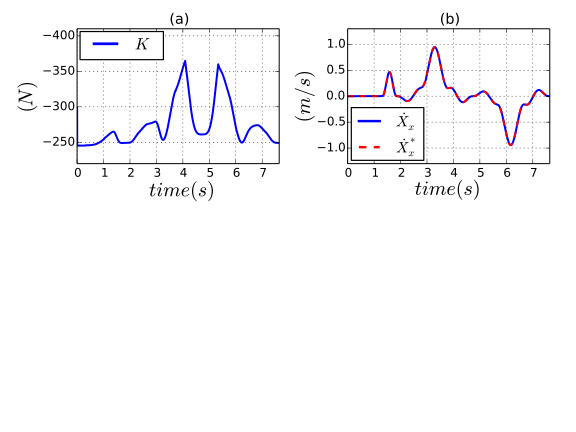
\includegraphics[width=1\columnwidth]{figures/k_xdot}}
\caption{(a) Producible braking force of the robot expressed at the level of its end-effector in the opposite direction to the considered obstacle (case $O_2$ in Fig.~\ref{fig:kuka_in_xde862301_a}). (b) are the instantaneous real and desired velocities along the $\vect{x}$ axis in Cartesian space.} 
\label{fig:k_xdot}
\end{figure}
Maximum tracking errors in Cartesian space are: $1 \times 10^{-3}~m$ for position and $2.3 \times 10^{-2}~rad$ for orientation. 
%%%%%$$$$$$$$$$$$$$$$$$
%Fig.~\ref{fig:q_qdot} shows how the limits on articular position, velocity, torque and also jerk are satisfied whenever a joint reaches its considered bounds. Along the movement of the robot, articular positions are within their max/min boundaries. 
%%%%%%%%%%%%%%%%%%%%%%%%%%%%%%%%%%%%%%%%%%%%%%%%%%%%%%%%%%%%%%%%%%%%%%%ù
%Along the movement of the robot, the limits on articular position, velocity, and also torque are satisfied whenever a joint reaches its considered bounds. 
%%%%%%%%%%%%%%%%%%%%%%%%%%%%%%%%%%%%%%%%%%%%%%%%%%%%%%%%%%%%%%%%%%%%%%ùù
%And thanks to the new formulation of the constraint on articular velocity ((\ref{eq:cnt_lit_22}) \& (\ref{eq:cnt_lit_22_bis})), the compatibility with the constraint on articular jerk (\ref{eq:cnt_lit_55}) is ensured. Indeed, when coping with a joint velocity limit (see joint $0$ in Fig.~\ref{fig:q_qdot}.b and Fig.~\ref{fig:tau_qdddot}.b), maximum producible jerk is used to bring the articular acceleration to zero. More details about this new formulation of the joint velocity constraint can be found in Chapter~\ref{chap:Constrcomp}, Subsection~\ref{subsec:jnt_vel_cnstr_inc_jerk}.
%%%%%%%%%%%%%%%%%%%%%%%%%%%%%%%%%%%%%%%%
%\begin{figure}[!htbp]
%\centering
%{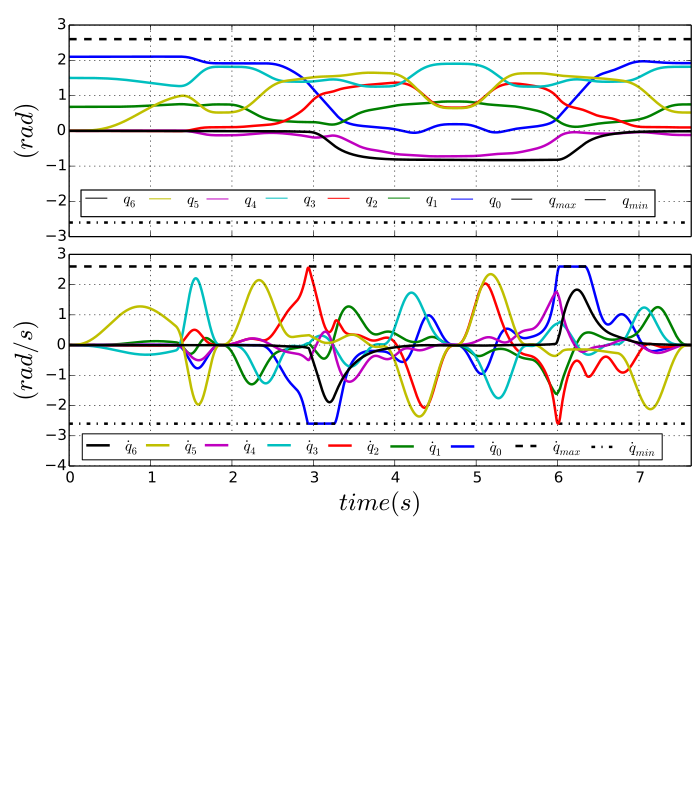
\includegraphics[width=0.90\columnwidth]{figures/q_qdot}}
%\caption{Articular position and velocity that correspond to the pick and place movement when the energy of the robot is not constrained.} 
%\label{fig:q_qdot}
%\end{figure}
%%%%%%%%%%%%%%%%%%%%%%
%\begin{figure}[!htbp]
%\centering
%{\includegraphics[width=0.8\columnwidth]{\figurepath/q}}
%\caption{4} 
%\label{fig:q}
%\end{figure}
%\begin{figure}[!htbp]
%\centering
%{\includegraphics[width=0.8\columnwidth]{\figurepath/qdot}}
%\caption{5} 
%\label{fig:qdot}
%\end{figure}
%\begin{figure}[!htbp]
%\centering
%{\includegraphics[width=0.8\columnwidth]{\figurepath/qdotdot}}
%\caption{6} 
%\label{fig:qdotdot}
%\end{figure}
%%%%%%%%%%%%%%%%%%%%%%%%%%%%%%%%%%%%
%\begin{figure}[!htbp]
%\centering
%{\includegraphics[width=0.90\columnwidth]{figures/tau_qdddot}}
%\caption{Articular torque and jerk that correspond to the pick and place movement when the energy of the robot is not constrained.} 
%\label{fig:tau_qdddot}
%\end{figure}
%%%%%%%%%%%%%%%%%%%%%%%%%%%%%%%%%
%\begin{figure}[!htbp]
%\centering
%{\includegraphics[width=0.8\columnwidth]{figures/tau}}
%\caption{7} 
%\label{fig:tau}
%\end{figure}
%\begin{figure}[!htbp]
%\centering
%{\includegraphics[width=0.8\columnwidth]{figures/qdotdotdot_!!!!}}
%\caption{8} 
%\label{fig:qdotdotdot_!!!!}
%\end{figure}
%\\
%\begin{figure}[h]
%\centering
%{\includegraphics[width=0.7\columnwidth]{figures/art_data_woO_woEc}}
%\caption{Articular positions, velocity and torque of the  pick and place movement without constraint on the kinetic energy of the end-effector.} 
%\label{fig:art_data_woO_woEc}
%\end{figure}
\\
The trajectory of the robot in this scenario does not intersect with any obstacle. During this \textit{free movement}, a number of parameters related to the dynamic capabilities of the robot in operational space and to the accomplished task are registered. Fig.~\ref{fig:k_xdot}.a illustrates the instantaneous producible equivalent braking force in Cartesian space expressed at the level of the end-effector in the opposite direction to the nearby obstacle (case $O_2$ in Fig.~\ref{fig:kuka_in_xde862301_a}). 

Kinetic energy of the KUKA LWR4, expressed at its end-effector and generated in the direction of the nearby considered obstacle (case $O_2$ in Fig.~\ref{fig:kuka_in_xde862301_a}) is shown in Fig.~\ref{fig:energy_profile}.a. Its maximum value is $2.15~J$.
At every time-step, the plotted kinetic energy is computed using two different formulations (\ref{eq:Ec_constr_first}) and (\ref{eq:Ec_eq_sum_Ep_a}).
%\begin{equation}
%S_c = E_{c_{|k}}^{EE,O} = \frac{1}{2} m(\vect{q}_{|k})_{EE,O}^{eq} v_{EE_{|k}}^{{EE,O}^2},
%\label{eq:plotted_Sc}
%\end{equation}
%and: 
%\begin{equation}
%\begin{split}
%S_c &= E_{c_{|k}}^{EE,O} = \sum\limits_{n=1}^{k-1} S_{p_{free_{|n}}} \\
%& =  \sum\limits_{n=1}^{k-1} m(\vect{q}_{|n})_{EE,O}^{eq} \ddot{X}_{EE_{|n}}^{EE,O} \left(\vect{X}_{EE_{|n+1}} - \vect{X}_{EE_{|n}}\right) \vect{n}_O.
%\end{split}
%\label{eq:plotted_Sc2}
%\end{equation}
Fig.~\ref{fig:energy_profile}.a illustrates how the kinetic energy of the robot at time-step $k$ is indeed equal (errors aside) to the sum of all the previously \textit{injected} energies.
%the small difference between the two curves is mainly due to the variation of the articular configuration between two successive control time-steps: $n$ and $n+1$; the Jacobian and equivalent mass are not considered at the same time-step.
\begin{figure}[!htbp]
\centering
{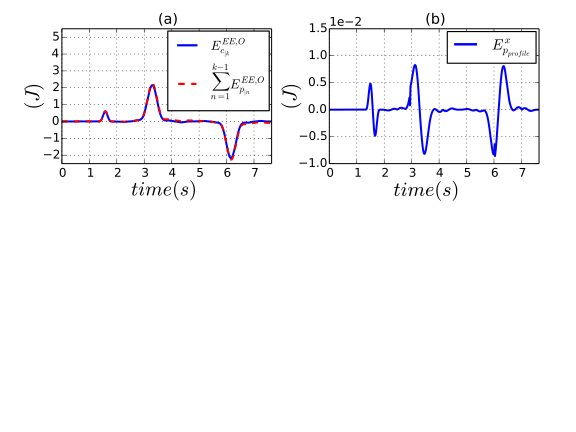
\includegraphics[width=1\columnwidth]{figures/energy_profile}}
\caption{(a) Kinetic energy of the robot in the direction of the considered obstacle (case $O_2$ in Fig.~\ref{fig:kuka_in_xde862301_a}), computed using (\ref{eq:Ec_constr_first}) and (\ref{eq:Ec_eq_sum_Ep_a}) during the pick and place movement. (b) the energy profiles that correspond to the pick and place task along the $\vect{x}$ axis in Cartesian space.} 
\label{fig:energy_profile}
\end{figure}

\subsection{Scenario 1: obstacle intersecting with the trajectory of the robot and no constraints on its kinetic nor controller energies} \label{subsec_no_constr_energy}
In this scenario, the obstacle intersects with the \circled{2}-\circled{3} segment of the pick and place movement (case $O_1$ in Fig.~\ref{fig:kuka_in_xde862301_a}). At collision, $1.66~J$ of kinetic energy are instantaneously dissipated (see Fig.~\ref{fig:ec_obst3!!!!}.a. 
%\begin{figure}[h]
%\centering
%{\includegraphics[width=0.5\columnwidth]{\figurepath/Ke_wO_wC_woEc}}
%\caption{Dissipation of the unconstrained kinetic energy of the robot end-effector in the direction of the considered obstacle during collision.} 
%\label{fig:Ke_wO_wC_woEc}
%\end{figure}
\begin{figure}[!htbp]
\centering
{
\includegraphics[width=1\columnwidth]{figures/ec_obst35!!!!}}
\caption{(a) Kinetic energy of the KUKA LWR4 expressed at the level of its end-effector in the direction of the considered obstacle during, at and after collision. (b) Constrained kinetic energy of the robot expressed at the level of its end-effector in the direction of the collided obstacle (case $O_1$ in Fig.~\ref{fig:kuka_in_xde862301_a}).} 
\label{fig:ec_obst3!!!!}
\end{figure}
According to (\ref{eq:Energydissipationmodel1}) and as can be seen in  Fig.~\ref{fig:ep__f_tau_!!!!}.b, this fast dissipation induces a large impact force of $551~N$. Which could clearly damage the collided obstacle or the robot. In this simulation and also in all the upcoming ones, a force sensor is linked to the base of the collided object. The main impact force is along the $\vect{x}$ axis (see Fig.~\ref{fig:kuka_in_xde862301_a}), which is the main direction of movement of the end-effector before collision.
% and thus, the controller can be considered unsafe.   
%\begin{figure}[!htbp]
%\centering
%{\includegraphics[width=0.8\columnwidth]{figures/force_sensor2}}
%\caption{10} 
%\label{fig:force_sensor2}
%\end{figure}
\begin{figure}[!htbp]
\centering
{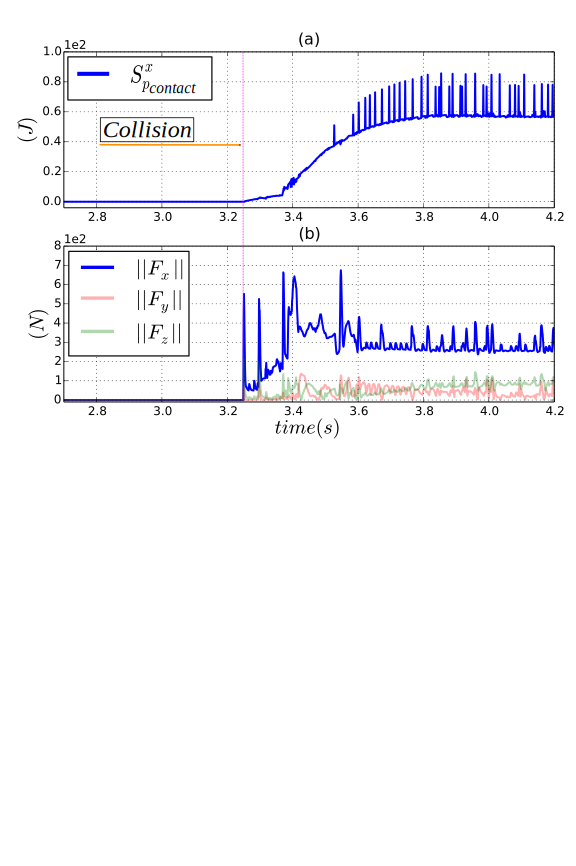
\includegraphics[width=0.95\columnwidth]{figures/ep__f_tau_!!!!}}
\caption{(a) \textit{Energy} accumulated in the controller of the robot during physical contact along the $\vect{x}$ axis in Cartesian space. (b) Contact forces between the robot and the wall after the establishment of physical contact along the $\vect{x}$, $\vect{y}$ and $\vect{z}$ axis in Cartesian space.} 
\label{fig:ep__f_tau_!!!!}
\end{figure}
After the peak of force corresponding to the first collision, physical contact between the robot and the wall is established. As this obstacle obstructs the movement of the KUKA LWR4, the divergence between the desired and real positions for its end-effector causes the augmentation of the amount of \textit{energy} that accumulates in the controller of the robot (see Fig.~\ref{fig:ep__f_tau_!!!!}.a). Consequently, the resulting contact force along the $\vect{x}$ axis also intensifies to reach $250~N$. The other collision peaks are caused by collisions between other parts of the robot and the wall. During physical contact, the constraint on the controller's accumulated \textit{energy} when expressed at the level of the end-effector, does not prevent the movement of other \textit{free} parts of the body of the robot. \\
%\begin{figure}[!htbp]
%\centering
%{\includegraphics[width=0.8\columnwidth]{figures/Ep_contact_selon_x_seul_!!!!}}
%\caption{11} 
%\label{fig:Ep_contact_selon_x_seul_!!!!}
%\end{figure}
%\begin{figure}[!htbp]
%\centering
%{\includegraphics[width=0.8\columnwidth]{figures/tau2}}
%\caption{12} 
%\label{fig:tau2}
%\end{figure}
The \textit{energy} that accumulates in the controller of the robot and the contact force derived from it stop increasing when the desired position for the end-effector stops diverging once at point \circled{3} from the \circled{2}-\circled{3} segment (see Fig.~\ref{fig:kuka_in_xde862301_a}).\\
Clearly, considering the big amounts of generated impact and contact forces, the controller with its current configuration is not appropriate for enabling \textit{safe} physical interaction between the robot and its environment. The introduced energy related constraints are then used in the upcoming scenarios.
%%%%%%%%%%%%%%%%%%%%%%%%%%%%%%%%%%%%%%%%%%%%%%%%%%%%%%%%%%%%
\subsection{Scenario 2: obstacle intersecting the trajectory of the robot and constraints on its kinetic and \textit{controller} energies}
Similarly to the previous scenario, the wall intersects with the \circled{2}-\circled{3} segment of the pick and place movement. As the robot moves, the second formulation of the constraint on kinetic energy (\ref{eq:Safe_constr_2_bis}) is included in the configuration of the controller and used to limit the amount of kinetic energy the robotic manipulator deploys in the direction of obstacle $O_1$. After the establishment of physical-contact, without removing the constraint on kinetic energy, the constraint (\ref{eq:Safe_constr_4_3_axisaaa}) is added to the controller and used to saturate the amount of \textit{energy} that accumulates in the controller. Articular inequality and equality constraints described in (\ref{eq:const_1}) and (\ref{eq:classic_constr_131}) are also considered in the control scheme. The parameters of the controller are fixed as: $E_{c_{safe}} = 0.05~J$, $K = 50~N$, $d_{safe} = 0.1~m$, $d_{max} = 0.3~m$ and $E_{p_{safe}}^{x} = 0.1~J$. During the physical-contact phase, contact forces applied by the robot to the wall are \textit{mainly} along the $\vect{x}$ axis. Consequently, only the \textit{controller energy} along this vector is constrained. 

Dissipated kinetic energy at collision is shown in Fig.~\ref{fig:ec_obst3!!!!}.b. As it is  pre-constrained, only $0.035~J$ of kinetic energy are dissipated at collision, resulting into an impact force of $85~N$ (see Fig.~\ref{fig:ep__f_tau65_!!!!}.b.
%\begin{figure}[!htbp]
%\centering
%{\includegraphics[width=0.75\columnwidth]{figures/dist_ec_ecmax_plot55}}
%\caption{Constrained kinetic energy of the robot expressed at the level of its end-effector in the direction of the collided obstacle (case $O_1$ in Fig.~\ref{fig:kuka_in_xde862301_a}).} 
%\label{fig:dist_ec_ecmax_plot55}
%\end{figure}
%\begin{figure}[!htbp]
%\centering
%{\includegraphics[width=0.8\columnwidth]{figures/force_sensor255}}
%\caption{10} 
%\label{fig:force_sensor255}
%\end{figure}
\begin{figure}[!htbp]
\centering
{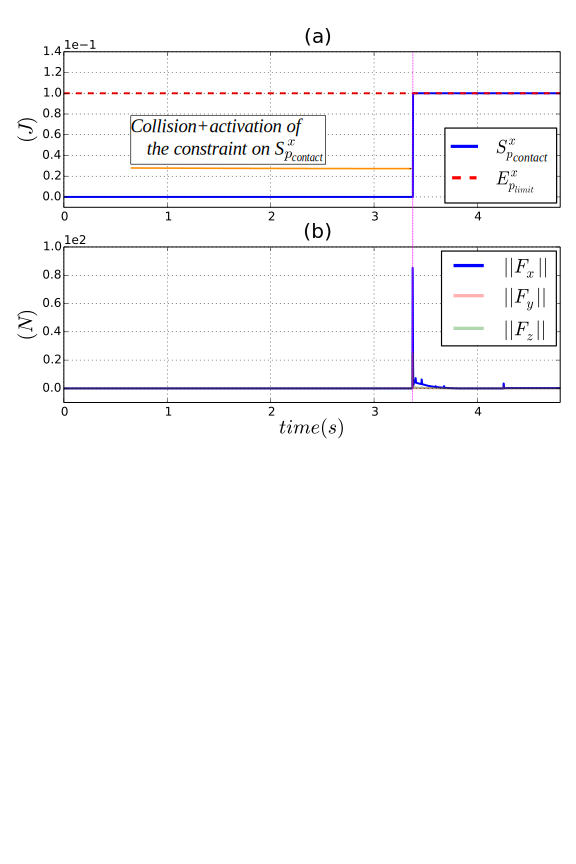
\includegraphics[width=0.95\columnwidth]{figures/ep__f_tau65_!!!!}}
\caption{(a) Constrained \textit{controller energy} stored in the controller of the robot during physical contact along the $\vect{x}$ axis in Cartesian space. (b) Corresponding contact forces along the $\vect{x}$, $\vect{y}$ and $\vect{z}$ axis in Cartesian space. (c) Actuation torques during the physical contact with the considered obstacle (case $O_1$ in Fig.~\ref{fig:kuka_in_xde862301_a}).} 
\label{fig:ep__f_tau65_!!!!}
\end{figure}
As shown in Fig.~\ref{fig:ec_obst3!!!!}~(b), using the second formulation (\ref{eq:Safe_constr_2_bis}), the constraint on kinetic energy is satisfied at every time-step, exactly the same as when the first formulation (\ref{eq:Ec_constr_a}) is used \cite{meguenani2015control}. On the other hand, Fig.~\ref{fig:ep__f_tau65_!!!!}.a shows how the constraint on the \textit{energy} that accumulates in the controller of the robot during physical-contact is also satisfied at every time-step.
%\begin{figure}[!htbp]
%\centering
%{\includegraphics[width=0.8\columnwidth]{\figurepath/ep_contact_selon_x_seul_!!!!55}}
%\caption{11} 
%\label{fig:ep_contact_selon_x_seul_!!!!55}
%\end{figure}
Because this \textit{energy} is saturated at a constant value $0.1~J$, the contact force derived from it decreases over time to reach $0~N$ (see Fig.~\ref{fig:ep__f_tau65_!!!!}.b) as the Cartesian tracking error between the real and desired positions for the end-effector of the robot increases. 

When using the current configuration of the controller, if any physical-contact is established between the robot and a human-operator, the manipulator can easily and safely be moved or pushed away.
%\begin{figure}[!htbp]
%\centering
%{\includegraphics[width=0.8\columnwidth]{figures/tau2555}}
%\caption{12} 
%\label{fig:tau2555}
%\end{figure}
%%%%%%%%%%%%%%%%%%%%%%%%%%SUBSECTION%%%%%%%%%%%%%%%%%%%%%%%%%%%%%
%%%%%%%%%%%%%%%%%%%%%%%%%%%%%%%%%%%%%%%%%%%%%%%%%%%%%%%%%%%%%%%%%
%%%%%%%%%%%%%%%%%%%%%%%%%%SUBSECTION%%%%%%%%%%%%%%%%%%%%%%%%%%%%%
\subsection{Scenario 3: obstacle intersecting with the trajectory of the robot and constraint on its task energy profile}
In this scenario, obstacle $O_1$ also intersects with the \circled{2}-\circled{3} segment of the pick and place movement. During the movement of the robot, its energy profile (described in Section~\ref{subsec:Task_energy_profile}) is constrained using (\ref{eq:Safe_constr_3_axis}). The kinetic energy of the robot is not constrained and the articular inequality and equality constraints respectively described in (\ref{eq:const_1}) and (\ref{eq:classic_constr_131}) are also included in the configuration of the controller. As shown in Fig.~\ref{fig:energy_profile}, based on the measured energy profiles along the $\vect{x}$, $\vect{y}$ and $\vect{z}$ axis, the  parameters of the controller are fixed as: $E_{p_{profile}}^{x}+\epsilon_{E_p}^{x} = 0.01~J$, $E_{p_{profile}}^{y}+\epsilon_{E_p}^{y} = 0.0045~J$ and $E_{p_{profile}}^{z}+\epsilon_{E_p}^{z} = 0.015~J$. With $\epsilon_{E_p}^{x}$, $\epsilon_{E_p}^{y}$ and $\epsilon_{E_p}^{z}$ used to compensate the repeatability related variations on the controller's \textit{energy} needed to accomplish the pick and place task.
%\footnote{According to the measured energy profiles in Fig.~\ref{fig:energy_profile}.b, Fig.~\ref{fig:energy_profile}.c and Fig.~\ref{fig:energy_profile}.d, \epsilon_{E_p}^{x}}. \\

As can be seen in Fig.~\ref{fig:x_x_dot454}, during the pre-collision phase, the tracking performances of the controller are not altered by the constraint on the \textit{task energy profile}. Indeed, during the \textit{free} movement of the robot, this constraint is never activated. The desired position, orientation and velocity for the end-effector are properly tracked, exactly the same as if this constraint is not included in the control scheme. \\
At collision, the desired position (also the velocity) for the end-effector starts diverging from its real value. Consequently, the \textit{energy} stored in the controller starts to increase and triggers the activation of the constraint on the \textit{task energy profile}. During physical contact, this constraint behaves exactly the same as (\ref{eq:Safe_constr_4_3_axisaaa}). According to Fig.~\ref{fig:ep_profil_xyz_futur_with_recnstruted6}, the \textit{controller energy} related constraint is successfully satisfied along the $\vect{x}$, $\vect{y}$ and $\vect{z}$ axis.
The peak of \textit{energy} along the $\vect{x}$ axis at collision is caused by the induced impact force. \\
Fig.~\ref{fig:ec__f_tau65_grand_!!!!}.a shows how $1.66~J$ of kinetic energy are dissipated at impact. Fig.~\ref{fig:ec__f_tau65_grand_!!!!}.b depicts the resulting collision  and contact force: $551~N$ are induced at the first impact. \\ 
Thanks to the constraint on the \textit{task energy profile} that has been included in the configuration of the controller, the resulting contact force is also reduced. The robot at this stage is compliant and can easily and safely be moved by a human-operator. 
\begin{figure}[!htbp]
\centering
{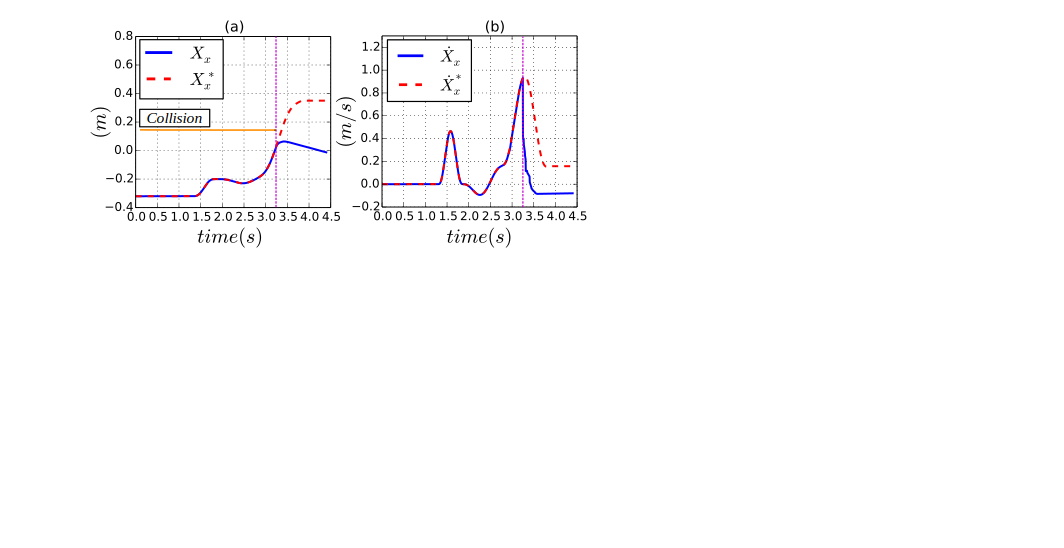
\includegraphics[width=0.99\columnwidth]{figures/x_x_dot454}}
\caption{(a) Real and desired position for the end-effector of the robot in Cartesian space as its task energy profile is constrained. (b) shows the real and desired velocity for the end-effector as the robot is submitted to the same constraint (case $O_1$ in Fig.~\ref{fig:kuka_in_xde862301_a}).} 
\label{fig:x_x_dot454}
\end{figure}
\begin{figure*}
\centering
{\includegraphics[width=2\columnwidth]{figures/ep_profil_xyz_futur_with_recnstruted6}}
\caption{Constrained energy profile for the pick and place task along the $\vect{x}$, $\vect{y}$ and $\vect{z}$ axis in Cartesian space.} 
\label{fig:ep_profil_xyz_futur_with_recnstruted6}
\end{figure*}
\begin{figure}[!htbp]
\centering
{\includegraphics[width=0.99\columnwidth]{figures/ec__f_tau65_grand_!!!!}}
\caption{(a) Kinetic energy of the robot expressed at the level of its end-effector as it physically interacts with the nearby obstacle (case $O_1$ in Fig.~\ref{fig:kuka_in_xde862301_a}). (b) Corresponding impact contact forces along the $\vect{x}$, $\vect{y}$ and $\vect{z}$ axis in Cartesian space.} 
\label{fig:ec__f_tau65_grand_!!!!}
\end{figure}
%\begin{figure}[!htbp]
%\centering
%{\includegraphics[width=0.8\columnwidth]{\figurepath/ec_obst6}}
%\caption{9} 
%\label{fig:ec_obst6}
%\end{figure}
%\begin{figure}[!htbp]
%\centering
%{\includegraphics[width=0.8\columnwidth]{\figurepath/force_sensor6}}
%\caption{11} 
%\label{fig:force_sensor6}
%\end{figure}
%\begin{figure}[!htbp]\centering
%{\includegraphics[width=0.8\columnwidth]{\figurepath/tau26}}
%\caption{12} 
%\label{fig:tau26}
%\end{figure}
%
%%%%%%%%%%%%%%%%%%%%%%%%%%%%%%%%%%%%%%%%%%
%%%%%%%%%%%%%%%%%%%%%%%%%%%%%%%%%%%%%%%%%%%%%%%
             %Rsults discussion and conclusion%
%%%%%%%%%%%%%%%%%%%%%%%%%%%%%%%%%%%%%%%%%%%%%%%%%%%%%%%%%
\section{Conclusion}
\label{sec:conslusion}
Human-robot interaction is one of the most complex scenarios a robotic system could face. Indeed, in such dynamic and non-predictable environment, several criteria must be satisfied with safety being the most important one. In the work presented in this paper, a new control strategy that allows the modulation of both the kinetic energy of the robot and the amount of \textit{energy} held in its controller is introduced. This approach is successfully used to ensure safety for the environment of the robot during interaction phases. The impact force at the establishment of a physical contact is reduced by monitoring then constraining the kinetic energy of a robotic arm under some \textit{safe} limit just before collision. The contact force on the other hand is diminished thanks to the constraint on the \textit{energy} that accumulates in the controller of the robot during physical-contact. Each constraint is composed of: 1) an introduced energy based safety indicator that reflects the degree of danger the robot represents towards the environment and, 2) an energy based safety criterion that corresponds to the amount of energy considered to be safe for the robot to exhibit during the interaction. \\
First used separately to express the energy based constraints, the relation between the robot's kinetic and controller energies is formulated and the robot along with its controller is represented as a system to which \textit{energy} is \textit{injected} and transformed into kinetic one. Based on this representation, the concept of \textit{task energy profile} is introduced. It represents the instantaneous amount of \textit{energy} held in the controller of the robot and that transforms into kinetic one during its free movements. For tasks with repetitive motion cycles, this profile is registered then used for the formulation of a constraint that saturates the instantaneous amount of \textit{energy} loaded in the controller and which is intended to increase in case of a deliberate or non-intentional physical contact with the environment. This results into a compliant robot that does not generate harmful contact forces. Illustrated on a KUKA LWR4 robotic arm in simulation, the introduced safe control strategy allows the robot to safely physically interact with its environment. On-going work focuses on the hardware integration of \textit{task energy profile} related constraint on a KUKA LWR4 serial robot to make it capable of safely interacting with a human operator entering its workspace.
%
%The energy based safety indicator proposed and validated in this paper holds a great potential for human/robot collaboration tasks. Indeed, energy is a universal component that can describe several physical phenomena linked to the physical interaction process. Velocity, inertia and also contact forces can all be expressed and modulated with this same quantity. Using the presented control framework and the introduced energy based criterion, the robot has been proven capable of producing different behaviours towards a nearby considered obstacle just by acting on physically meaningful  control parameters. During its motion, at every time-step, the kinetic energy of the  end-effector is controlled. If a collision occurs or contact with the environment is desired, the dissipated energy is modulated to smooth the interaction process  and guarantee safety for both the robot and the obstacle. Enabling/disabling contact and stopping the robot at a desired distance from the obstacle are different behaviours that can be obtained using the same controller.
%
%%Besides being computationally heavy, an other issue to be dealt with while using a QP formulation for the robot controller is the constraints expression. Indeed, changing from an unconstrained phase to a constrained one will generated discontinuities in the computed torque of the system. Thus, linear and quadratic constraints formulation must be revised.  
%
%On-going work focuses on the hardware integration of the presented control framework and safety criterion on a Kuka LWR4 serial robot. The distance between the end-effector and the human operator is acquired with a 3D visual system, here a Microsoft Kinect, and encouraging preliminary results have been obtained as illustrated on Fig.~\ref{fig:experiment}. The reliability and continuity of the measured distance is still to be improved and the velocity of the human operator must be considered. The Gurobi QCQP solver is running as an Orocos component on a Linux operating system patched with Xenomai to ensure proper real-time constraints at $1~kHz$. Given the computational load induced by the QCQP, a $1~kHz$ sampling frequency cannot be guaranteed yet and the overall performances have to be improved.  
%
%Besides the improvement of the computational aspects of the control problem, future work  will focus  on the potential energy part of the safety criterion.  The  $(kinetic~+~potential)$ energy exchange  between the robot and its environment still has to be studied, validated in simulation and integrated on the real robot.
\bibliographystyle{IEEEtran}
\bibliography{IEEEabrv,IROS_PAPER_Vincent_V2}


\end{document}
